% ======================================================================
% Inicio del preámbulo 
% ======================================================================

\documentclass[12pt,letterpaper]{article}
\usepackage[left=2cm, top=2.5cm, bottom=2.5cm, right=2cm]{geometry}
\usepackage[spanish]{babel}
\selectlanguage{spanish}

\usepackage[utf8]{inputenc} % Reconocimiento de tildes y otros caracteres
\usepackage{graphicx}
\usepackage{setspace}
\usepackage[scaled]{helvet}
\renewcommand\familydefault{\sfdefault}
\usepackage[justification=centering]{caption}
\usepackage[labelfont=bf]{caption}
\usepackage {amsmath, amssymb, multicol, cancel} % cargar librerías para fórmulas símbolos y otras cosas
\usepackage{placeins}
\usepackage{float} % forzar la figura en la subsección que le corresponde
\usepackage{pdfpages}

\addto\captionsspanish{\renewcommand{\tablename}{Tabla}} % Cambiar nombre a tablas

\usepackage{hyperref} % permite agregar links
\hypersetup{
    colorlinks=true,
    linkcolor=black,
    urlcolor=blue,
    citecolor=black,
    } % características de los links

\def \imgwidth {150mm} % ancho de las figuras

% ======================================================================
% Fin del preámbulo 
% ======================================================================

\begin{document}

\begin{titlepage}
\begin{center}
\textbf{UNIVERSIDAD DE COSTA RICA}\\ 
\vspace{6mm}
\textbf{ESCUELA DE INGENIERÍA ELÉCTRICA}\\
\vspace{3cm}
\textbf{IE0624}\\
\textbf{Laboratorio de Microcontroladores}\\
\vspace{3cm}
\textbf{Proyecto Final}\\
\vspace{0.5cm}
Sistema de suministro de agua y comida controlado por IoT\\
\vspace{3cm}
Estudiantes:\\
Kendall Saborio Picado - B87103\\
Alexander Rojas Brenes - B86869\\
\vspace{1.5cm}
Profesor:\\
Ing. Marco Villalta Fallas
\vfill
Fecha de entrega: 04/07/2024
\end{center}
\end{titlepage}

\tableofcontents

\newpage
\section{INTRODUCCIÓN}

Este proyecto se centra en el desarrollo de un dispensador de comida y agua para mascotas con capacidades IoT, el proyecto ha sido un esfuerzo integral para crear una solución automatizada y eficiente para el cuidado de las mascotas. Este sistema utiliza sensores ultrasónicos para monitorear los niveles de comida y agua, y permite a los propietarios controlar y supervisar el dispensador a través de una aplicación móvil, utilizando la plataforma Blynk.

Durante el desarrollo del proyecto, se realizaron ajustes significativos en el diseño y la selección de componentes para cumplir con las prioridades definidas. La adaptación a las limitaciones técnicas, como el cambio de motores y la búsqueda de alternativas, permitió avanzar en el desarrollo del dispensador, logrando así el objetivo principal del proyecto.

A lo largo del proceso, se enfrentaron varios problemas técnicos, como la falta de potencia del ESP8266 y dificultades con Arduino Cloud. Para superar estos obstáculos, se implementaron estrategias efectivas, incluyendo la transición a la plataforma Blynk, lo que garantizó el funcionamiento del sistema de dispensación de comida y agua. Esto demostró una notable flexibilidad y capacidad de resolución de problemas.

Se logró implementar funcionalidades básicas de IoT mediante la integración de Blynk, permitiendo el monitoreo remoto del estado de los recipientes y el control del sistema desde un dispositivo móvil. Esta implementación cumplió parcialmente con el objetivo de automatización del suministro, facilitando el control a distancia del sistema.

La construcción del hardware, que incluye el dispensador de comida, el sistema de bombas para agua y los sensores ultrasónicos, fue completada exitosamente. Este aspecto del proyecto proporcionó una base sólida para el funcionamiento básico del sistema, permitiendo que el dispensador cumpliera con sus funciones principales de manera efectiva.

Para consultar el trabajo realizado, puede consultarse el siguiente repositorio de trabajo, en la rama llamada ``Proj'': \url{https://github.com/SaboEIE/IE-0624_IS_2024_B87103/tree/Proj}. El código principal en C (archivo .ino), puede consultarse en la ruta \path{Proj/src}. 

\section{JUSTIFICACIÓN}
Este proyecto busca mejorar el bienestar animal al garantizar que las mascotas y animales de granja reciban los nutrientes necesarios en los momentos adecuados. Además, ofrece una solución conveniente para los propietarios, especialmente aquellos con horarios ocupados, al automatizar el proceso de alimentación y liberarlos de la preocupación por mantener horarios específicos de alimentación. El uso de tecnología conectada a Internet permite el monitoreo remoto de la alimentación de los animales, lo que resulta especialmente útil y permite a los propietarios estar ausentes durante largos períodos de tiempo. Además, la automatización del suministro de comida y agua facilita el control preciso del consumo, evitando el desperdicio y garantizando un suministro adecuado sin excesos. 

\section{OBJETIVOS}

\subsection{Objetivo general}
Diseñar y desarrollar un dispositivo suplidor inteligente de agua y comida para animales utilizando ESP8266, con el fin de mejorar el bienestar animal y proporcionar una solución conveniente para los propietarios, automatizando el proceso de alimentación y permitiendo el monitoreo remoto de la alimentación de los animales.

\subsection{Objetivos específicos}

\begin{enumerate}
    \item Implementar un sistema de suministro de agua y comida que permita tanto la solicitud directa del usuario como una rutina automatizada con tiempos predefinidos, utilizando tecnología ESP8266 para controlar los mecanismos de dispensación.
    \item Integrar la aplicación Arduino Cloud para enviar notificaciones al teléfono móvil del usuario, informando sobre el contenido de los recipientes y los tanques principales de agua y comida, así como para permitir la programación de suministros automáticos y solicitudes adrede.
    \item Garantizar un control preciso del consumo de comida y agua mediante la automatización del suministro, evitando el desperdicio y asegurando un suministro adecuado sin excesos. 
\end{enumerate}
 

\newpage
\section{NOTA TEÓRICA}

Antes de iniciar con el desarrollo del presente proyecto, es necesario tener a mano una serie de conceptos importantes, los cuales se explican a continuación: 

\subsection{Placa NODEMCU ESP8266 WIFI}

La placa NodeMCU ESP8266 es una plataforma de desarrollo muy accesible y de bajo costo, basada en el microcontrolador ESP8266. Este microcontrolador de 32 bits utiliza la arquitectura Tensilica Xtensa LX106 y puede operar a una frecuencia de entre 80 MHz y 160 MHz. Una de sus características más destacadas es su capacidad Wi-Fi integrada, lo que permite que la placa se conecte a redes Wi-Fi y funcione tanto como punto de acceso como cliente, lo que la hace ideal para proyectos de Internet de las Cosas (IoT).

La NodeMCU ESP8266 ofrece 17 pines GPIO (General Purpose Input/Output) para conectar sensores, actuadores y otros periféricos (4 pueden configurarse como PWM a 3.3V). También incluye pines para comunicación I2C, SPI, UART, ADC, entre otros. Su programación es muy accesible, ya que puede hacerse usando el entorno de desarrollo Arduino IDE, lo que la hace ideal para principiantes y entusiastas. Además, puede programarse en lenguaje Lua a través del firmware NodeMCU.

El microcontrolador ESP8266 cuenta con una memoria flash interna, de 4 MB, que permite almacenar el firmware y otros datos necesarios para el funcionamiento del dispositivo. Gracias a sus capacidades Wi-Fi y su bajo costo, la NodeMCU ESP8266 es utilizada en una amplia variedad de proyectos, desde la automatización del hogar hasta sistemas de monitoreo remoto y dispositivos IoT.

La placa puede ser alimentada mediante un cable micro-USB o a través de los pines de alimentación (VIN y GND), con un voltaje de funcionamiento de 3.3V. Además, es compatible con plataformas de desarrollo como Blynk, facilitando la creación de aplicaciones móviles para controlar y monitorear dispositivos conectados.

A continuación se puede ver el Diagrama de pines de la placa:

\begin{figure}[H]
\centering
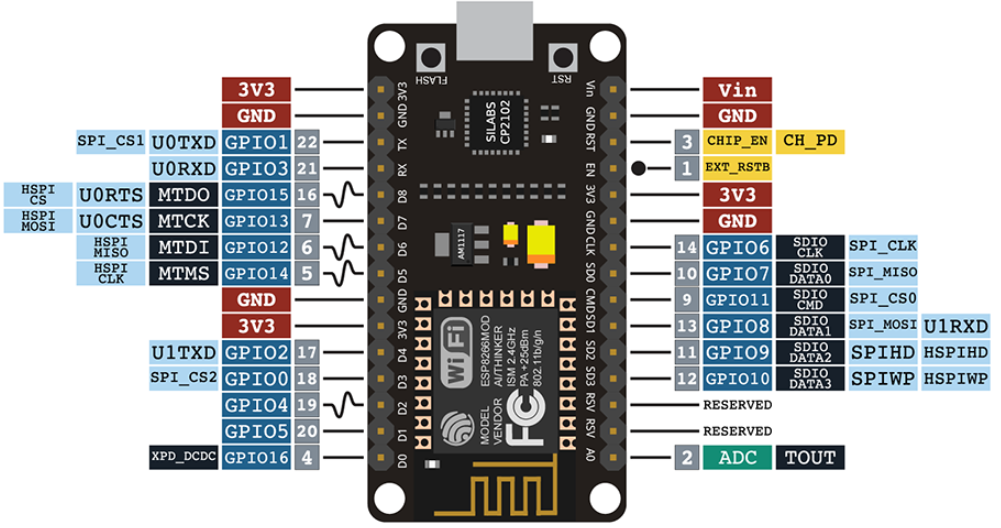
\includegraphics[width=120mm]{./Figuras/Nota_teorica/PINOUT_PLACA}
\caption{Diagrama de Pines NodeMCU ESP8266. (Fuente: \cite{Acrobotic_2016})}
\label{fig:HC}
\end{figure}

\subsubsection{Características Eléctricas: ESP8266}
A continuación se muestran las caracteristicas electricas del ESP8266 según su hoja del fabricante \cite{EspressifSystems_2023}:

\begin{table}[H]
    \centering
    \scriptsize
    \begin{tabular}{|l|l|c|c|c|c|}
        \hline
        \textbf{Parameters} & \textbf{Conditions} & \textbf{Min} & \textbf{Typical} & \textbf{Max} & \textbf{Unit} \\ \hline
        Operating Temperature Range & - & -40 & Normal & 125 & C \\ \hline
        Maximum Soldering Temperature & IPC/JEDEC J-STD-020 & - & - & 260 & C \\ \hline
        Working Voltage Value & - & 2.5 & 3.3 & 3.6 & V \\ \hline
        $V_{IL}$ & - & -0.3 & - & 0.25 $V_{IO}$ & V \\ \hline
        $V_{IH}$ & - & 0.75 $V_{IO}$ & - & 3.6 & V \\ \hline
        $V_{OL}$ & - & - & - & 0.1 $V_{IO}$ & V \\ \hline
        $V_{OH}$ & - & 0.8 $V_{IO}$ & - & - & V \\ \hline
        $I_{max}$ & - & - & - & 12 & mA \\ \hline
        Electrostatic Discharge (HBM) & TAMB = 25  C & - & - & 2 & KV \\ \hline
        Electrostatic Discharge (CDM) & TAMB = 25  C & - & - & 0.5 & KV \\ \hline
    \end{tabular}
    \caption{Características eléctricas NodeMCU ESP8266}
    \label{table:nodemcu_parameters}
\end{table}
\subsubsection{Diagrama de bloques: ESP8266}
A continuación se muestra el Diagrama de bloques del ESP8266 según su hoja del fabricante \cite{EspressifSystems_2023}:

\begin{figure}[H]
\centering
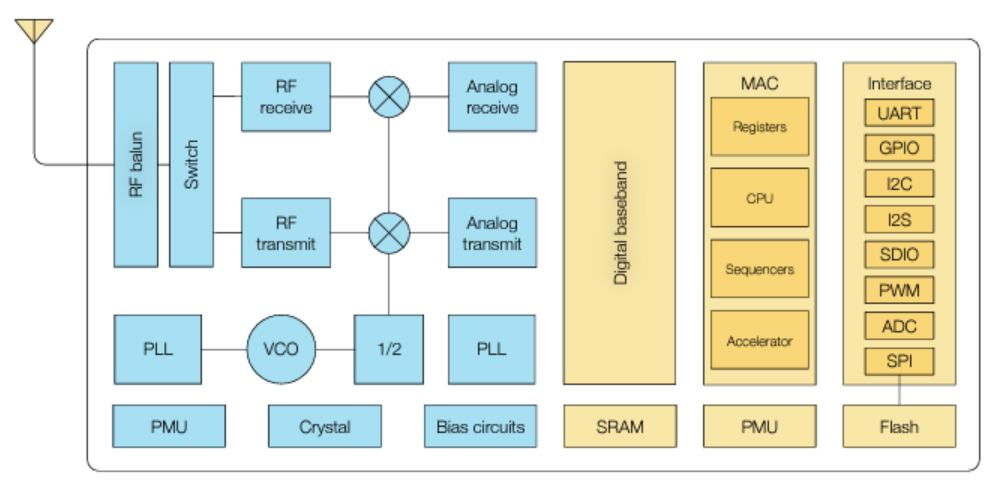
\includegraphics[width=120mm]{./Figuras/Nota_teorica/Diagrama_de_bloques_micro}
\caption{Diagrama de bloques ESP8266. (Fuente: \cite{EspressifSystems_2023})}
\label{fig:esp1}
\end{figure}

\subsection{Librerías de importancia}
A continuación se detallan las librerías que fueron utilizadas en el proyecto:

\begin{itemize}
    \item \underline{\texttt{ESP8266WiFi.h}}: permite al ESP8266 conectarse a redes WiFi. Proporciona funciones para escanear redes disponibles, conectar o desconectar de una red, y obtener información sobre la conexión actual, como la intensidad de la señal y la dirección IP asignada.
    
    \item \underline{\texttt{BlynkSimpleEsp8266.h}}: diseñada para integrar el ESP8266 con la plataforma Blynk. Permite conectar el dispositivo a la aplicación móvil Blynk para crear interfaces de usuario con botones, \textit{sliders} y otros \textit{widgets} para controlar el ESP8266 y recibir datos en tiempo real.

    \item \underline{\texttt{Servo.h}}: permite controlar servomecanismos con el ESP8266. Proporciona funciones para configurar el ángulo del servo motor, establecer la velocidad de movimiento, y otras operaciones básicas necesarias para controlar servos en proyectos de robótica o automatización.
\end{itemize}

\subsection{IoT: Internet of things}
El Internet de las cosas (IoT, por sus siglas en inglés) se refiere a una red abierta y completa de objetos inteligentes que tienen la capacidad de autoorganizarse, compartir información, datos y recursos, reaccionando y actuando ante situaciones y cambios en el entorno. Es un concepto que ha evolucionado desde la idea de que la primera versión de Internet trataba sobre datos creados por personas, mientras que la siguiente versión se trata de datos creados por cosas \cite{madakam2015internet}. 

\subsection{Sensores ultrasónicos (HC-SR04)}
El HC-SR04 es un sensor de distancia ultrasónico que se destaca por su bajo costo y facilidad de uso. Este sensor es capaz de medir distancias en un rango de 2 cm a 400 cm, lo que lo convierte en una herramienta popular en proyectos de robótica y automatización para evitar obstáculos y medir distancias \cite{HC}. A continuación se detallan los pasos del funcionamiento del sensor: 

\begin{enumerate}
    \item \textbf{Emisión de onda ultrasónica}: el sensor está equipado con dos transductores ultrasónicos: uno para enviar las ondas (transmisor) y otro para recibirlas (receptor). Cuando se activa el pin Trig (\textit{Trigger}) enviando un pulso alto de al menos 10 µs, el sensor emite una serie de ondas ultrasónicas a una frecuencia de 40 kHz.

    \item \textbf{Reflexión de onda}: las ondas ultrasónicas viajan a través del aire y se reflejan en un objeto situado frente al sensor.

    \item \textbf{Recepción de onda}: el transductor receptor detecta las ondas reflejadas y genera un pulso en el pin Echo. La duración de este pulso es proporcional al tiempo que tardaron las ondas en viajar al objeto y regresar al sensor.

    \item \textbf{Cálculo de distancia}: La distancia se calcula utilizando la siguiente fórmula: 

    \begin{equation*}
        Distancia (d) = \frac{V \times T}{2}
    \end{equation*}

    Donde $V$ es es la velocidad del sonido en el aire y $T$ es el tiempo medido en microsegundos ($\mu$s) desde el envío hasta la recepción de las ondas.
\end{enumerate}

En la Figura \ref{fig:HC}, puede consultarse el comportamiento descrito, además de la disposición de pines: 

\begin{figure}[H]
\centering
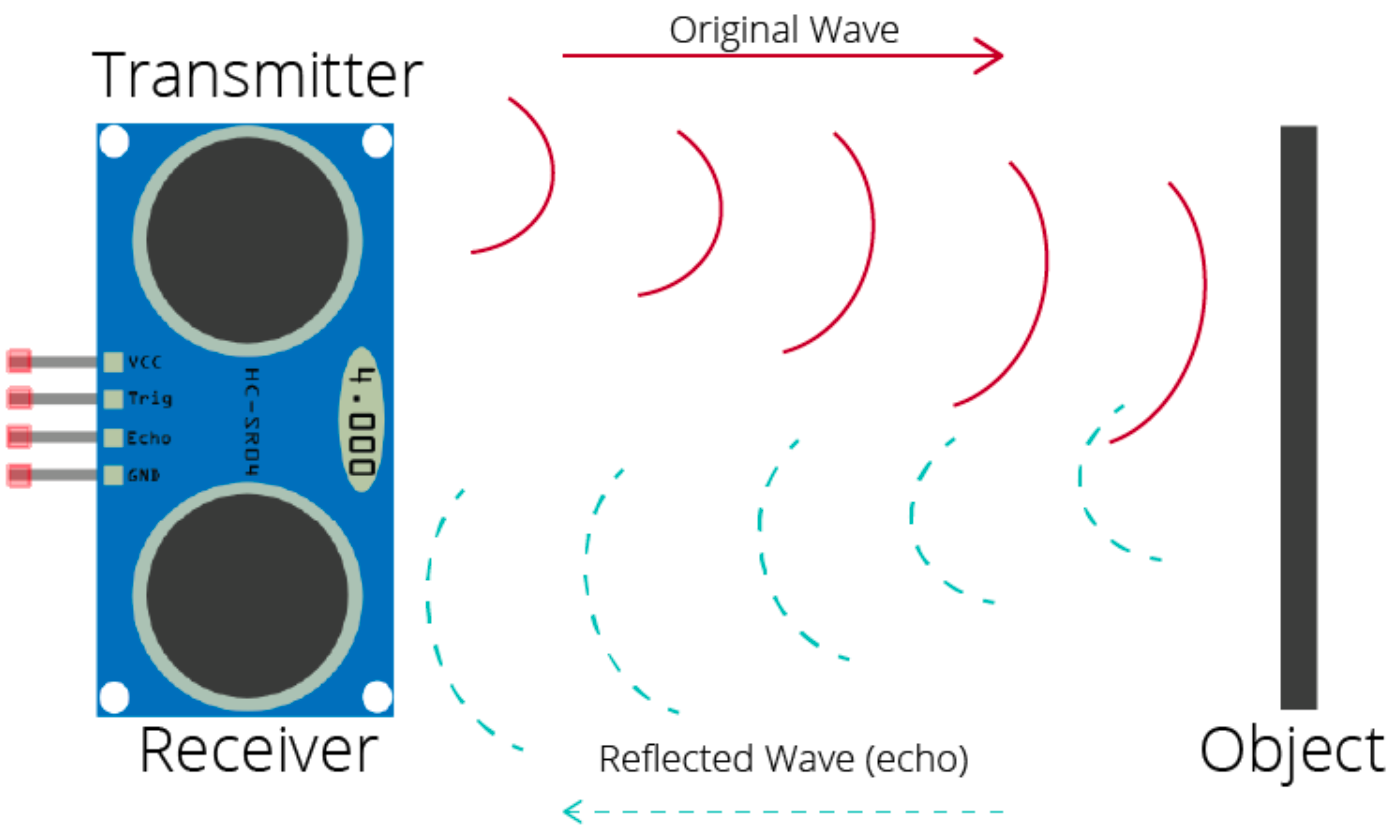
\includegraphics[width=120mm]{./Figuras/Nota_teorica/HC}
\caption{Funcionamiento del sensor ultrasónico HC-SR04 y disposición de pines del dispositivo. (Fuente: \cite{RNT})}
\label{fig:HC}
\end{figure}

\subsection{Servo motor del kit de Arduino}
Según se detalla en \cite{SM}, un servomotor es un dispositivo de actuador utilizado en diversos campos como la robótica, vehículos RC y modelos aéreos. Se destaca por su capacidad de control preciso de posición, lo que lo hace adecuado para tareas que requieren movimientos exactos y de alta fuerza. 

Un servomotor típico está compuesto por un motor eléctrico, un potenciómetro, electrónica de control y una caja de engranajes. El potenciómetro mide la posición actual del eje, y la electrónica de control compara esta posición con la posición deseada, ajustando el motor para mantener la posición del eje en el valor objetivo. Este proceso de ajuste continuo constituye un sistema de control en bucle cerrado. Lo anterior puede apreciarse de manera gráfica en la Figura \ref{fig:SM}: 

\begin{figure}[H]
\centering

\includegraphics[width=120mm]{./Figuras/Nota_teorica/SM}
\caption{Composición de un servo motor. (Fuente: \cite{SM})}
\label{fig:SM}
\end{figure}

Para conectar un servomotor a un microcontrolador, se deben conectar tres cables: alimentación (VCC) a 5V, tierra (GND) a GND, y señal a un pin digital del dispositivo de control. Es fundamental considerar que, si se utilizan múltiples servos o servos de mayor tamaño, se debe utilizar una fuente de alimentación externa para evitar dañar el microcontrolador.

\subsection{Bomba de agua}
Tal como se describe en \cite{BA}, este componente cuenta con un motor de 6V y 0.25A de alta resistencia, un cuerpo de plástico termoplástico resistente, y es completamente sumergible, aunque también puede funcionar en seco sin dañarse. La bomba, opera a un rango de voltaje de 2.5 a 6V, ofrece una elevación máxima de 40 a 110 cm y un caudal de 80 a 120 L/h. Sus dimensiones son un diámetro de aproximadamente 24 mm, una longitud de 45 mm y una altura de 33 mm. Equipado con un motor magnético sin escobillas y una vida útil de 500 horas de funcionamiento continuo, este dispositivo es ideal para aplicaciones diversas como fuentes, cascadas, y sistemas de riego automatizados, garantizando un movimiento eficiente y confiable del agua. En la Figura \ref{fig:WP}, puede observarse el tipo de mini bomba de agua que se utilizará en el proyecto: 

\begin{figure}[H]
\centering
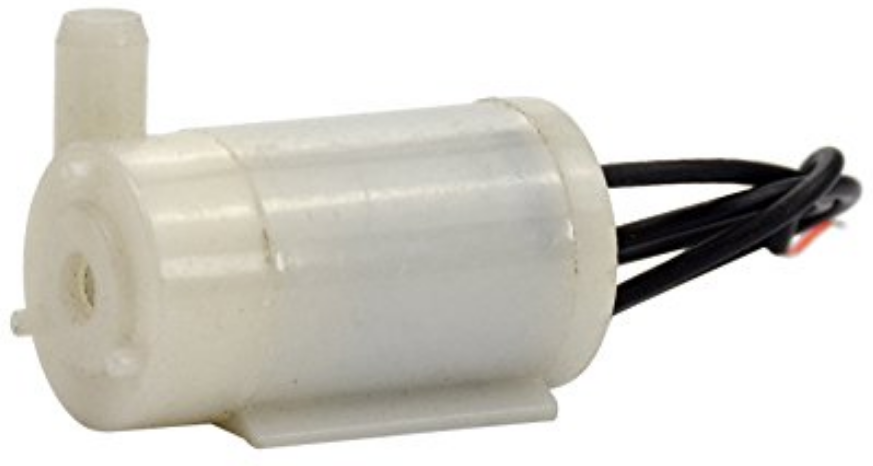
\includegraphics[width=100mm]{./Figuras/Nota_teorica/WP}
\caption{Mini-bomba de agua. (Fuente: \cite{BA})}
\label{fig:WP}
\end{figure}

Una bomba de agua funciona mediante un impulsor que gira para crear una fuerza centrífuga, lo que genera una baja presión en el centro y succiona el agua hacia el interior de la bomba a través del puerto de succión. El agua es entonces empujada hacia afuera mediante la presión generada y dirigida a través del puerto de descarga gracias al diseño de la voluta. El motor impulsa el impulsor, y en algunos casos, la bomba necesita ser primada para eliminar el aire y asegurar un flujo continuo de agua \cite{ST}.

\subsection{Blynk IoT}

Tal como se explica en \cite{BK}, Blynk es una plataforma en la nube para IoT de bajo código que simplifica la creación, implementación y gestión de aplicaciones IoT. Permite construir aplicaciones móviles y web personalizables sin necesidad de programación, gestionar dispositivos, datos y actualizaciones, y garantizar seguridad empresarial en todo el ciclo de vida del IoT. Blynk puede ser conectado con varios dispositivos como SP32, ESP8266, Arduino Uno, Raspberry Pi, Particle Photon, Seeed Wio Terminal y TI CC3220 y ofrece diversos métodos para conectar dispositivos a su plataforma en la nube:

\begin{itemize}
    \item \textbf{Blynk Library}: Una biblioteca C++ que proporciona una conexión bidireccional de baja latencia entre el dispositivo y la nube de Blynk, manteniendo el dispositivo siempre conectado.

    \item \textbf{Blynk.Edgent}: Una solución empaquetada que incluye Blynk.Inject para provisión dinámica de credenciales y Blynk.Air para actualizaciones de firmware OTA, ideal para hardware compatible con esta opción.

    \item \textbf{Blynk.NCP}: Una pila de software para módulos de procesamiento de red (NCP) que maneja la conectividad (WiFi, Ethernet, Celular), permitiendo al MCU principal usar una biblioteca cliente ligera para la comunicación.

    \item \textbf{HTTP(s) API}: Un protocolo estándar que permite a los dispositivos conectarse periódicamente a la nube para transferir datos, ideal para dispositivos celulares que envían datos en lotes.

    \item \textbf{MQTT API}: Un protocolo de comunicación bidireccional seguro que admite autenticación, actualizaciones de datos, eventos y más, ideal para proyectos que utilizan bibliotecas MQTT o plataformas similares.
\end{itemize}

Estos métodos ofrecen flexibilidad en el desarrollo y gestión de aplicaciones IoT, adaptándose a diferentes necesidades y tipos de hardware \cite{BK}.

\subsection{Lista de componentes y precios}
En la Tabla \ref{table:Equipo} pueden consultarse los componentes utilizados y sus precios tomando como referencia los precios del sitio web de la tienda de componentes MicroJPM (\url{https://www.microjpm.com/}): 

\begin{table}[H]
\caption{Lista de componentes.}
\begin{center}
\begin{tabular}{c|c|c}
\hline
\textbf{Componente}&\textbf{Cantidad}&\textbf{Precio}\\
\hline
NodeMCU ESP8266 & 1 & \$10,95\\
Batería de 9 V & 1 & \$5.64\\
Servo motor & 1 & \$5,95\\
Mini bomba agua sumergible & 1 & \$5,50\\
Resistor de  2 k$\Omega$ & 2 & \$0,80\\
Transistor 2N2222 & 1 & \$0,25\\ 
Relé & 1 & \$1.08\\
Diodo & 1 & \$0.095\\ 
Jumpers & 60 & \$6.90\\
Materiales de construcción & - & \$11.71\\
Mano de obra & - & \$19.99\\
\hline
Total & - & \$68.86\\
\end{tabular} \label{table:Equipo}
\end{center}
\end{table}

% Poner el precio en colones

Según la Tabla \ref{table:Equipo}, para realizar este proyecto son necesarios ₡36176.15, según el valor del dólar al momento de escribir el presente informe. 

\newpage
\section{DESARROLLO Y ANÁLISIS DE RESULTADOS}
A continuación se muestran los métodos de desarrollo utilizados para resolver cada uno de los problemas planteados, así como la funciones utilizadas, el \textit{hardware} construido y los resultados obtenidos:

\subsection{Desarrollo de la solución}
En esta sección, se explica el proceso de desarrollo de \textit{hardware} y \textit{software} utilizado para diseñar e implementar la solución planteada para el proyecto: 

%-----Harware-------
% Dispensador de comida/Servo/Stepper
\subsubsection{Dispensador de comida/Servo/Stepper}
Inicialmente se realizó una búsqueda de posibles diseños existentes para tomar ideas y construir el dispensador de comida.

\begin{figure}[H]
\centering
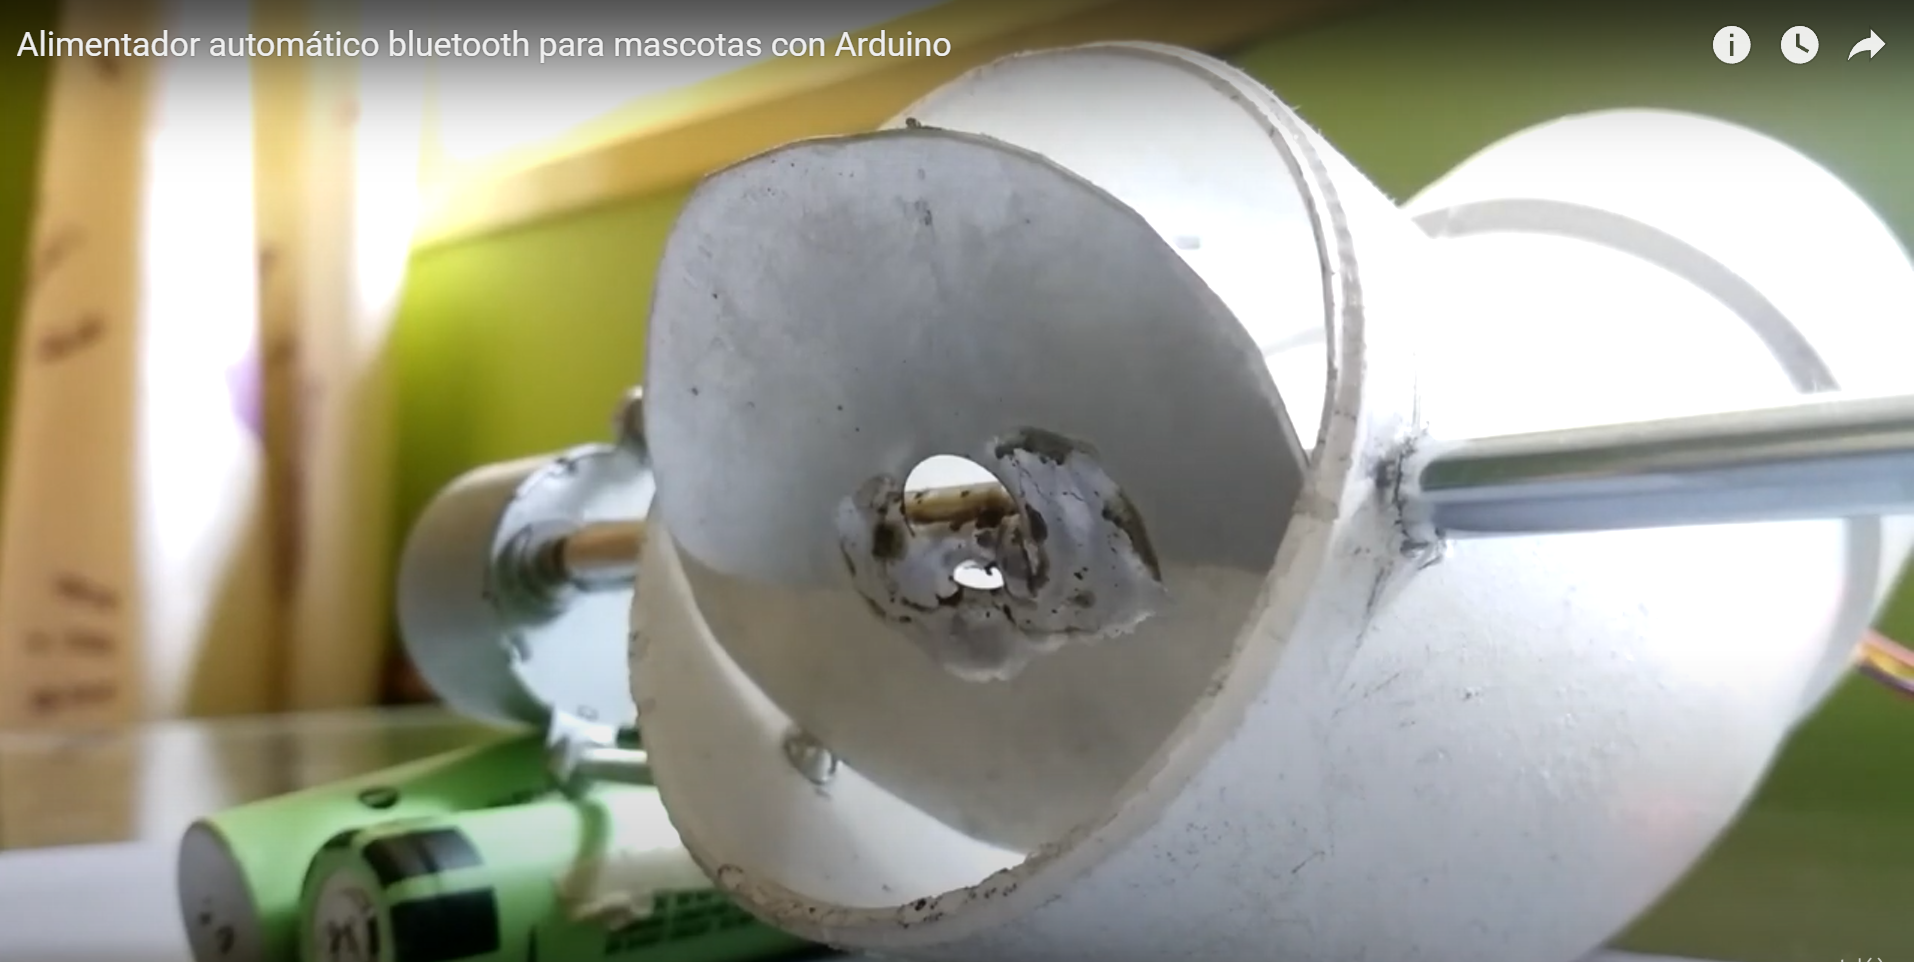
\includegraphics[width=90mm]{./Figuras/Desarrollo_Analisis/Diseño1}
\caption{Primer diseño consultado. (Fuente: \cite{TD_2019})}
\label{fig:DC}
\end{figure}

Este primer diseño es muy interesante, note que hace uso de un stepper motor así como de una especia de varille que controla la tapa de apertura del contenedor. Inicialmente se implementó uno diseño prácticamente idéntico, sin embargo un aspecto importante a considerar era que en el escenario de este proyecto, se desea que el reservorio principal tenga alimento para más de un refill. Esto generaba que la cantidad e alimento fuera considerable y que su peso cayera sobre la integridad de la tapa. Por que la tapa al intentar abrir, necesitaba el torque necesario para levantar el alimento. Al seguir consultando diseños propuestos, se encontró el siguiente:

\begin{figure}[H]
\centering
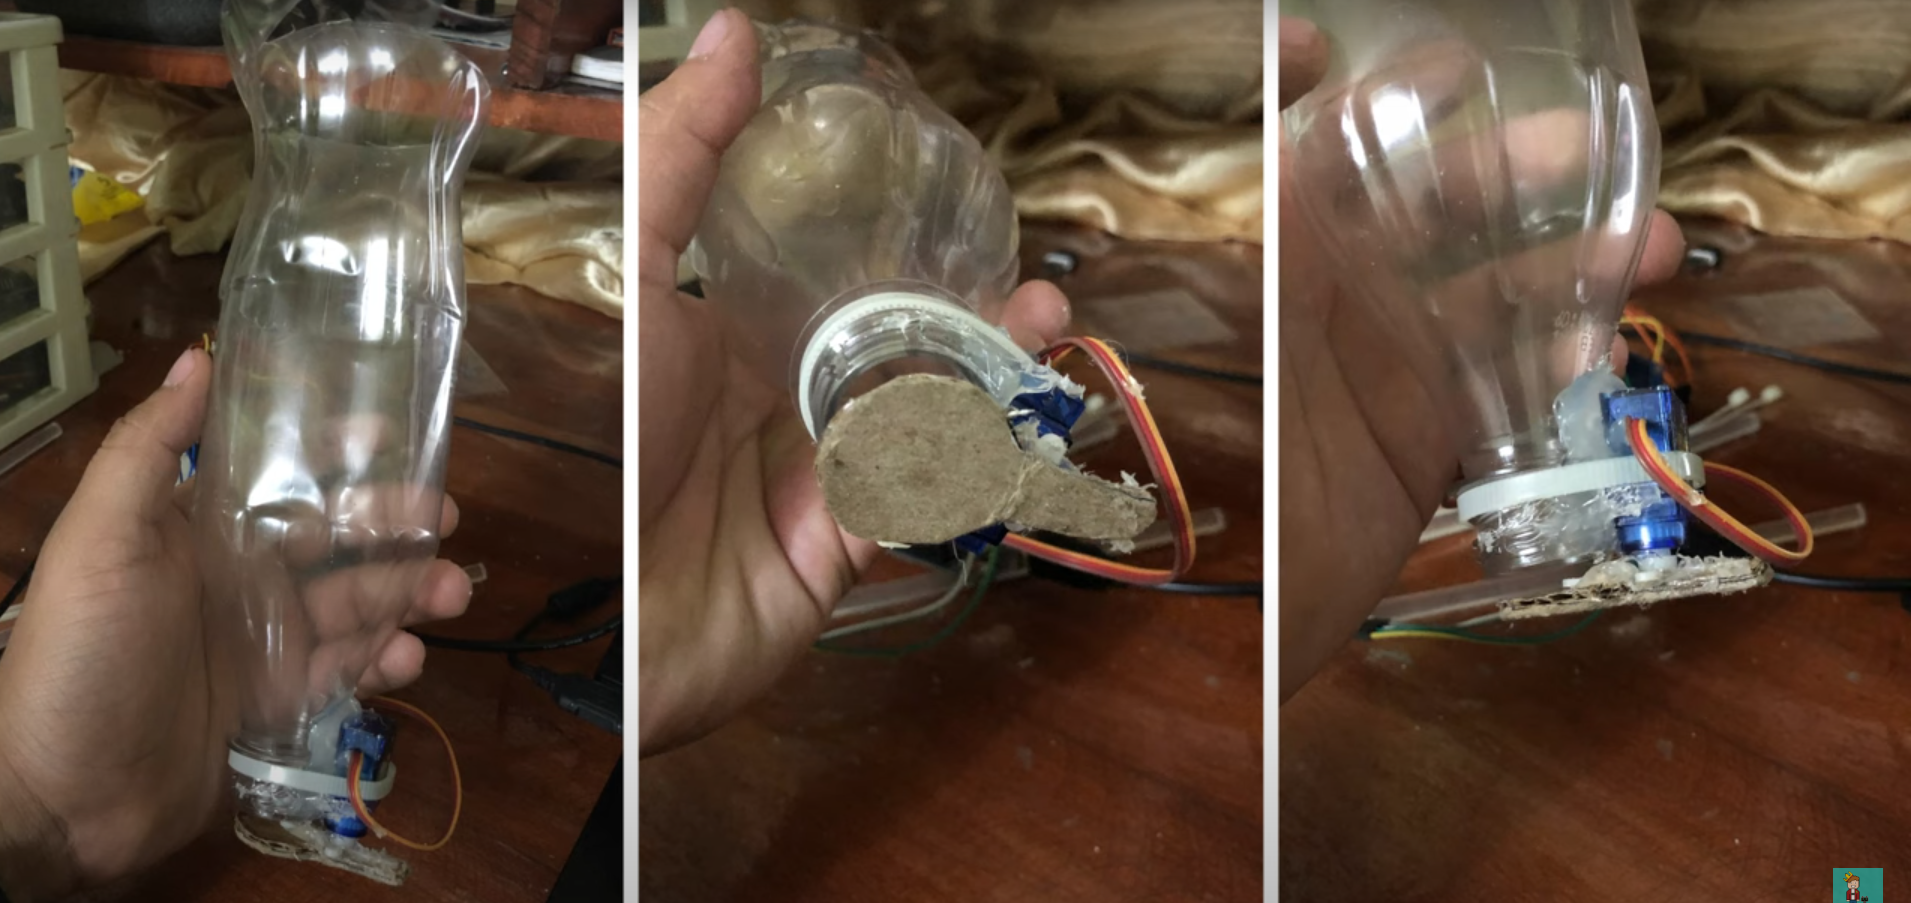
\includegraphics[width=90mm]{./Figuras/Desarrollo_Analisis/Diseño2}
\caption{Segundo diseño consultado. (Fuente: \cite{SalvaTronic_2024})}
\label{fig:DC2}
\end{figure}
De este diseño lo que resultó llamativo fué el uso del servomotor. Por lo qué de aca surgió la idea de migrar al uso de servo y crear una especia de portón corredizo que permitiera el flujo de comida. Para este portón se utilizó una malla reciclada, que normalmente se encuentra en la base de los sartenes de cocina. El diseño propuesto de dispensador de alimento para este trabajo el siguiente:

\begin{figure}[H]
\centering
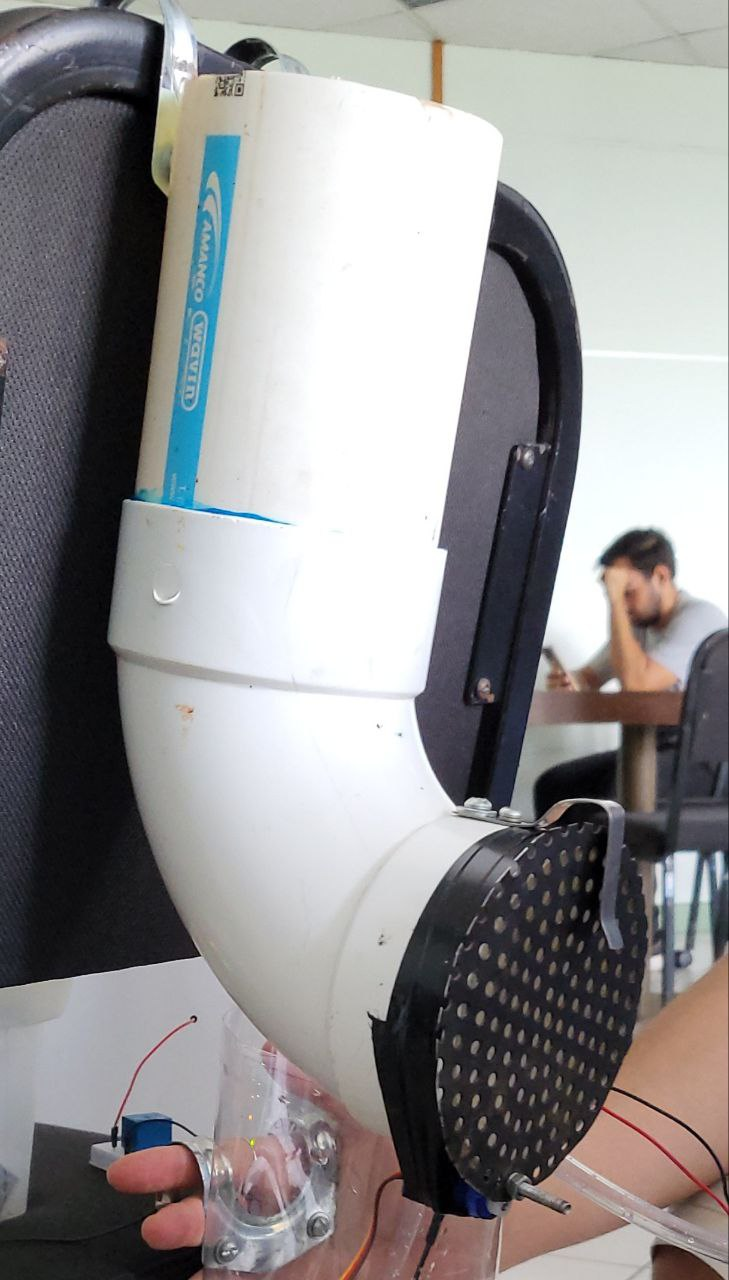
\includegraphics[scale=0.3]{./Figuras/Desarrollo_Analisis/diseño_final_dispensador_comida}
\caption{Diseño propuesto.}
\label{fig:DC3}
\end{figure}
Note que el diseño propuesto es una combinación de las ideas consultadas, más mejoras como por ejemplo el aumento de capacidad de almacenamiento pegando más tubo al codo. Se añadió una placa metálica plateada de seguridad, que mantiene la tapa del reservorio presionada, evitando así cualquier desperdicio o fuga de alimento. Note que se esta usando el servomotor, es importante mencionar que inicialmente se realizaron pruebas de funcionamiento usando Arduino con sus pines de 5V. Sin embargo una vez se consiguió el microcontrolador ESP8266 que es el microcontrolador seleccionado para este proyecto, este solo cuenta con pines 3.3v y menos corriente. Por lo que se percibió una disminución en el rendimiento y velocidad de operación del servomotor.


% Dispensador de agua/Bomba/Rele/Transistor
\subsubsection{Dispensador de agua/Bomba/Relé/Transistor}
Para lo que es el reservorio de agua, se decidió utilizar una botella plástica esto por disponibilidad del material, su naturaleza resistente a los líquidos y su capacidad de almacenaje. En ambos reservorios tanto de comida como de agua, se añadió un soporte, que permite apoyar los reservorios a cualquier tipo de silla o mueble.

\begin{figure}[H]
\centering
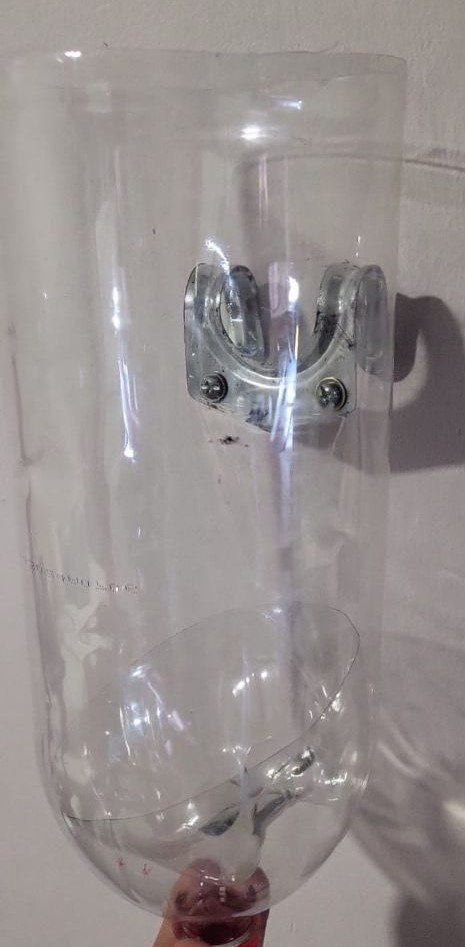
\includegraphics[scale=0.3]{./Figuras/Desarrollo_Analisis/reservorio_agua}
\caption{Imagen del Reservorio de agua con soporte.}
\label{fig:botella}
\end{figure}

Se obtuvo una bomba de agua del tipo sumergible, que no cuenta con alguna patilla de control. Por lo que se vió la necesidad de proponer un circuito de control con relé. Inicialmente antes de tener el ESP8266, se realizaron simulaciones y pruebas con el pin de alimentación de arduino UNO de 3.3 V, en el que se lograba activar el relé. Sin embargo al momento de migrar al ESP8266, el relé no ese activaba a pesar de tener la misma tensión. En este momento al consultar la literatura nos damos cuenta que los pines GPIO del ESP8266 tienen una corriente de salida de hasta 12 mA, mientras que los de Arduino de hasta 40 mA en este momento se percibe que es un problema por baja corriente. Investigando se encontró el circuito propuesto en \cite{Sergio_2020}, el cual resuelve este problema: 

\begin{figure}[H]
\centering
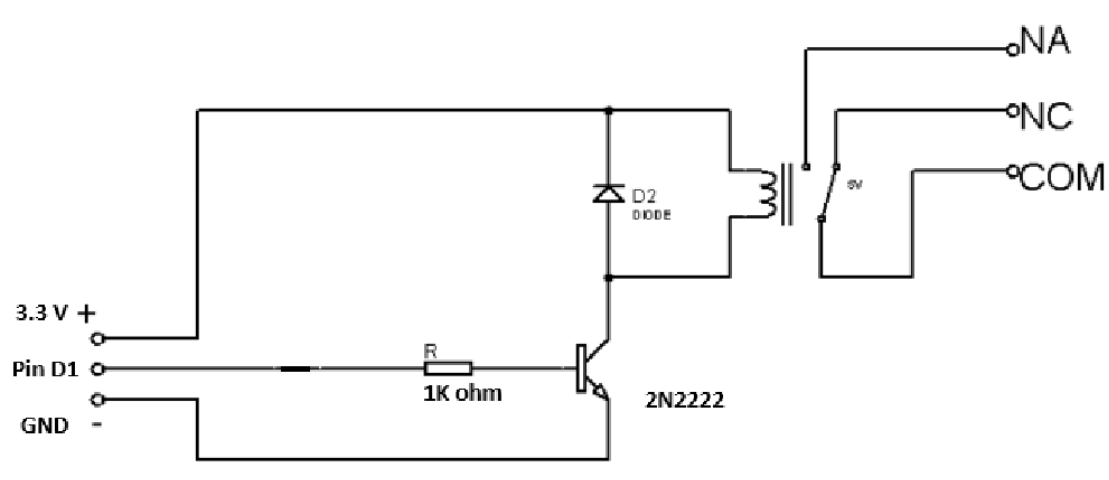
\includegraphics[scale=0.5]{./Figuras/Desarrollo_Analisis/Circuito_rele}
\caption{Imagen del Reservorio de agua con soporte.}
\label{fig:botella2}
\end{figure}

El uso de un transistor 2N2222 permite tener control sobre el relé usando una patilla GPIO del ESP8266 en la base del transistor. Así como elevar la corriente debido a la ganancia que poseen los transistores. El diodo se utiliza como protección a los picos generados en las transiciones del relé. De esta manera se logró realizar el control de la bomba con ESP8266.
\\
Un problema interesante que surgió en el bombeo entre el reservorio principal y la taza de agua del animal fué un fenómeno denominado como sifón. Un sifón es una diferencia de presión que permite que el agua fluya de un nivel más alto a uno más bajo, incluso sin la ayuda de la bomba.\cite{palomino2017analisis} Este fenomeno hacia que el agua fluyera hacia la taza del animal aun cuando la bomba se apagaba. La solución planteada fué variar la altura del reservorio principal.


\subsubsection{Tazas de agua y comida/Sensores ultrasónicos}
Para realizar las mediciones de distancia en las tazas de comida y agua, fue necesario colocar los sensores ultrasónicos en la parte superior de estas. Para fijar el sensor y evitar movimientos verticales y horizontales que insertaran ruido a las mediciones de nivel, se utilizó porcelana fría, la cual representa un buen material en la medida en que seca bastante rápido y evita cualquier movimiento. En la Figura \ref{fig:TS}, puede verse la forma en la que los sensores fueron colocados en cada taza:

\begin{figure}[H]
\centering
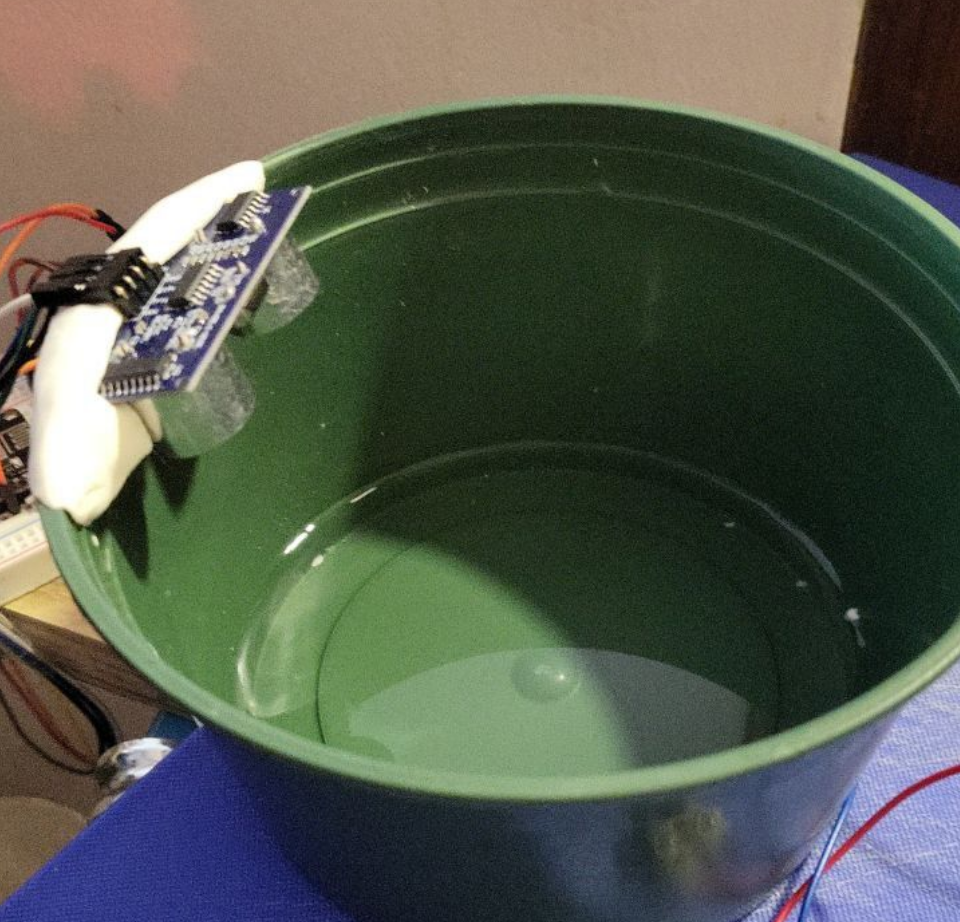
\includegraphics[width=90mm]{./Figuras/Desarrollo_Analisis/TS}
\caption{Taza de agua con el sensor ultrasónico adherido a este utilizando porcelana fría.}
\label{fig:TS}
\end{figure}

\subsubsection{Circuito general}
Una vez que se tenían todas las partes completadas, solamente restaba unir todas estas utilizando el microcontrolador elegido para el proyecto. En la Figura \ref{fig:CG} puede consultarse de manera general y a alto nivel el circuito construido:  

\begin{figure}[H]
\centering
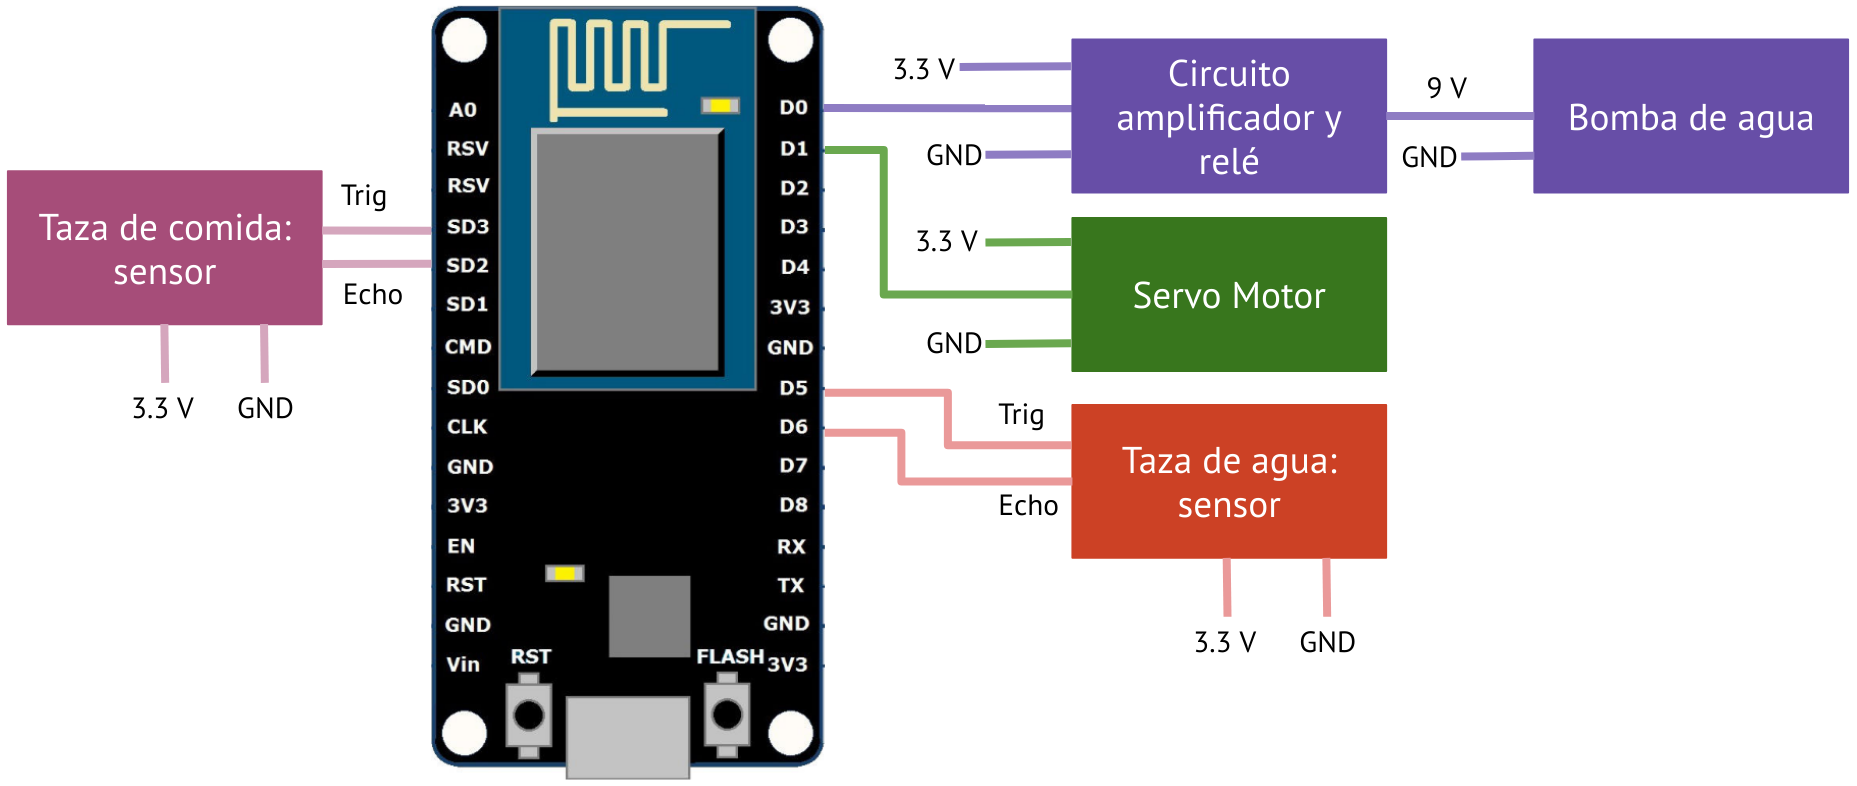
\includegraphics[width=155mm]{./Figuras/Desarrollo_Analisis/CG}
\caption{Disposición general del circuito utilizado para el proyecto. (Elaboración propia).} 
\label{fig:CG}
\end{figure}

Como puede verse en la Figura \ref{fig:CG}, el circuito está dividido en tres etapas: 
\begin{enumerate}
    \item \textbf{Tazas de agua y de comida}: cada un cuenta con un sensor ultrasónico que se encarga de la medición de proximidad del alimento y agua, resultando en un monitoreo constante del nivel en ambos casos. 

    \item \textbf{Servo motor}: este motor es controlador por el ESP8266, permite la distribución de comida en la taza de comida, cuando sea necesario. El motor tiene el objetivo de abrir el portón del contenedor principal de comida. 

    \item \textbf{Bomba de agua}: esta sección cuenta con dos partes. En primer lugar se tiene el circuito amplificador de corriente para poder accionar el relé de activación de la bomba de agua, este es alimentado por el ESP8266. En segundo lugar, se tiene la bomba de agua como tal, la cual se encargar de la distribución de agua desde el contender principal a la taza de agua cuando sea necesario. 
\end{enumerate}
A continuación se muestra el circuito completo conectado en su etapa de pruebas:
\begin{figure}[H]
\centering
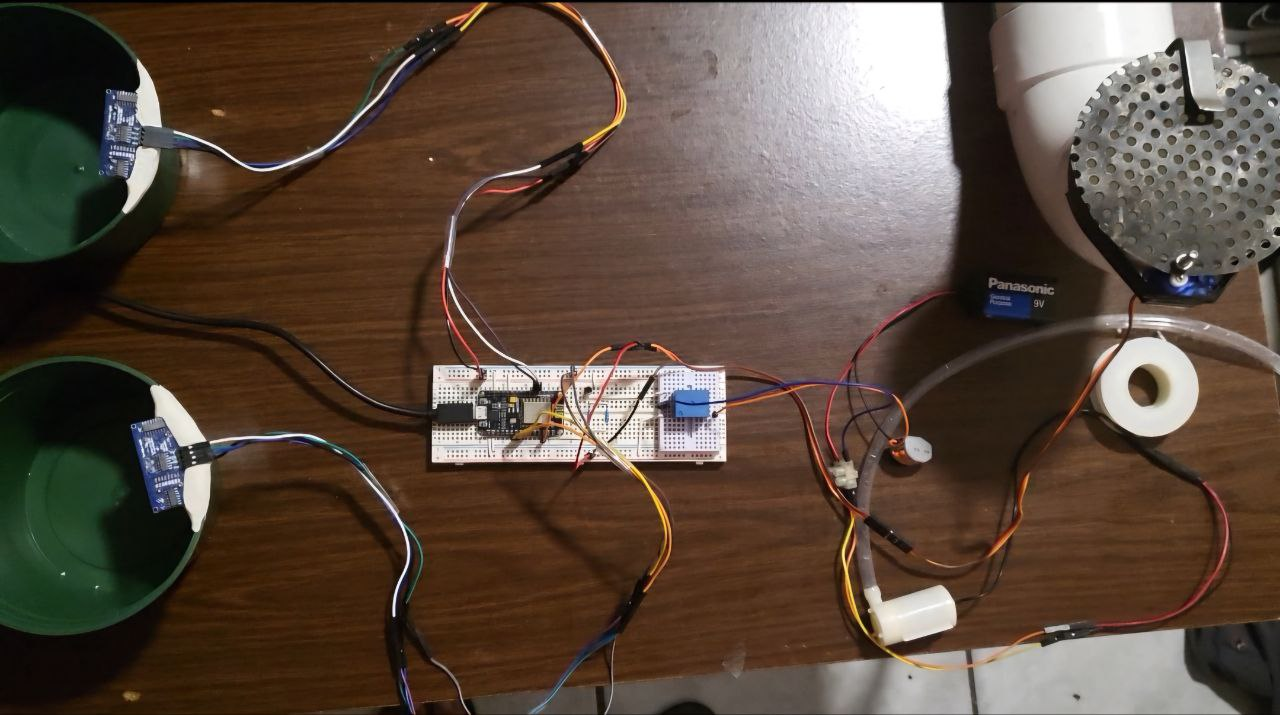
\includegraphics[width=155mm]{./Figuras/Desarrollo_Analisis/CG2}
\caption{Imagen del circuito completo en su etapa de pruebas. (Elaboración propia).} 
\label{fig:CG2}
\end{figure}

%-----Software------
\subsubsection{Desarrollo de \textit{software}}
A continuación podrá consultarse una descripción de alto nivel de cada una de las funciones implementadas en el código .ino:

\begin{itemize}
    \item \textbf{\texttt{setup()}}: esta corresponde a la función principal de configuración, en esta se configuran las siguientes partes: 
    \begin{itemize}
        \item \textbf{\texttt{setup\_servo()}}: se encarga de la configuración básica del servo motor. 
        \item \textbf{\texttt{setup\_pump()}}: se encarga de la configuración básica de los pines de control utilizados para controlar el circuito de amplificación que a su vez se encarga de controlar la bomba de agua.  
        \item \textbf{\texttt{setup\_ultrasonic()}}: configura los pines de de \textit{trigger} y \textit{echo} de los dos sensores ultrasónicos utilizados.  
    \end{itemize}

    \item \textbf{\texttt{distance\_measure(int trigPin, int echoPin)}}: esta función envía un pulso de 10 microsegundos al pin de disparo del sensor ultrasónico (trigPin), y luego mide el tiempo que tarda en recibir el pulso reflejado en el pin de eco (echoPin). Utiliza esta duración para calcular y retornar la distancia en centímetros.

    \item \textbf{\texttt{water\_level\_bowl(int trigPin, int echoPin)}}: mide la distancia desde el sensor ultrasónico ubicado en la taza de agua. Si la distancia medida es mayor o igual a 7 cm, se considera que la taza está vacía y se muestra un mensaje en el serial. Si se recibe una señal de Blynk para llenar la taza, la bomba de agua se activa hasta que la distancia medida sea menor a 4 cm. Durante este proceso, se envían los valores de nivel de agua a la aplicación Blynk.

    \item \textbf{\texttt{food\_level\_bowl(int trigPin, int echoPin)}}: mide la distancia desde el sensor ultrasónico ubicado en la taza de comida. Si la distancia medida es mayor o igual a 7 cm, se considera que la taza está vacía y se muestra un mensaje en el serial. Si se recibe una señal de Blynk para llenar la taza, el servo motor se mueve a 180 grados para dispensar comida hasta que la distancia medida sea menor a 5.5 cm. Durante este proceso, se envían los valores de nivel de comida a la aplicación Blynk.

    \item \textbf{\texttt{status\_checker()}}: verifica los niveles en las tazas de comida y agua. 

    \item \textbf{\texttt{loop()}}: Mantiene la conexión con el servidor de Blynk mediante \texttt{Blynk.run()}, gestionando la comunicación con la aplicación móvil. Además, llama a \texttt{status\_checker()} para monitorear y controlar los niveles de comida y agua en los recipientes y contenedores, tomando acciones en consecuencia.
\end{itemize}

\subsubsection{Arduino Cloud/Blynk}
Tal como había sido planteado al inicio del proyecto, se quería utilizar la plataforma Arduino Cloud para manejar el sistema construido utilizando IoT. A pesar de que se configuró e intentó la implementación de esta, se presentaron varios problemas:

\begin{itemize}
    \item Errores al intentar conectar el ESP8266 a la plataforma. A pesar de que el agente necesario fue instalado, la plataforma no era capaz de identificar el dispositivo todo el tiempo, lo que causaba inestabilidad al momento de hacer \textit{upload}.

    \item En las ocasiones en las que el dispositivo sí pudo conectarse a la plataforma, se tuvieron problemas con la conexión WiFi. El error correspondía a un problema con el \textit{broker} de  MqTT, ya que no podía acceder al puerto dispuesto para la comunicación, independientemente de la red en la que el dispositivo se conectara. 
\end{itemize}

Es por lo anterior que se decidió utilizar cambiar de plataforma y utilizar Blynk para realizar las mismas tareas planteadas para Arduino Cloud. La conexión entre la plataforma Blynk y el ESP8266 se logra mediante la función \texttt{Blynk.begin(auth, ssid, pass)}, que establece la conexión con el servidor de Blynk utilizando credenciales definidas. Dentro del bucle principal \texttt{loop()}, se llama continuamente a \texttt{Blynk.run()} para mantener activa la conexión y permitir la comunicación bidireccional. Los comandos y datos se intercambian a través de funciones como \texttt{BLYNK\_WRITE(V0)} y \texttt{BLYNK\_WRITE(V1)}, que responden a los cambios en los widgets de la aplicación, permitiendo controlar remotamente el nivel de comida y agua en las tazas.

\subsection{Análisis de los resultados}

% CASO A foto tazas vacías X / Impresion de terminal X / Foto de Dashboard X
\subsection{Caso A: Tazas Vacías}
A continuación se analiza el escenario en el que ambas tazas se encuentran vacías.

\begin{figure}[H]
\centering
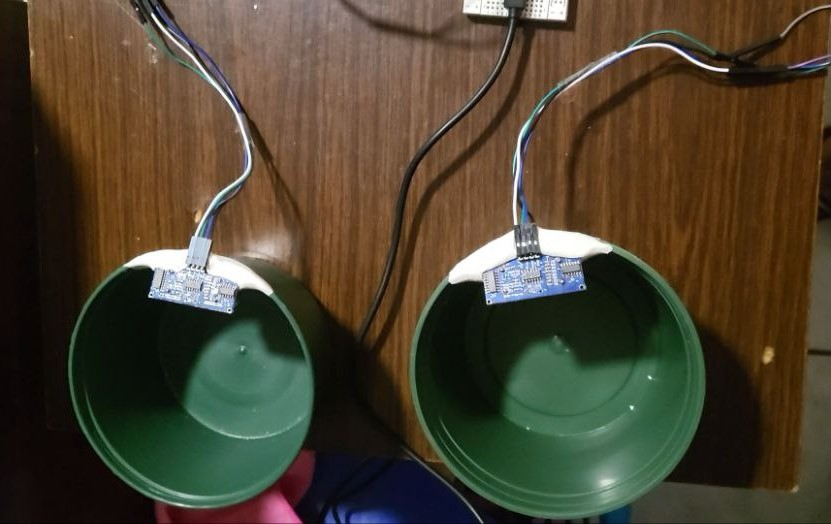
\includegraphics[width=110mm]{./Figuras/Desarrollo_Analisis/tazas_vacias}
\caption{Imagen del dispensador con las tazas vacías.} 
\label{fig:analisis1}
\end{figure}

En este escenario se espera que en terminal se realice la impresión que indique que tanto la taza de agua como la de comida se encuentran vacías. A continuación se muestra como efectivamente se cumple lo anterior:

\begin{figure}[H]
\centering
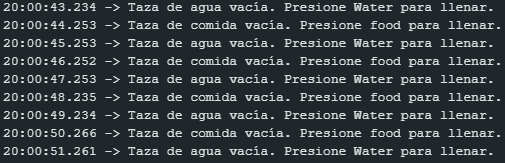
\includegraphics[width=100mm]{./Figuras/Desarrollo_Analisis/vacios}
\caption{Impresión en Serial monitor con las tazas vacías.} 
\label{fig:analisis2}
\end{figure}

Además se obtiene en el \textit{dashboard} de Blynk, que los niveles de las tazas reflejen valores bajos de acuerdo a su condición de vacíos:

\begin{figure}[H]
\centering
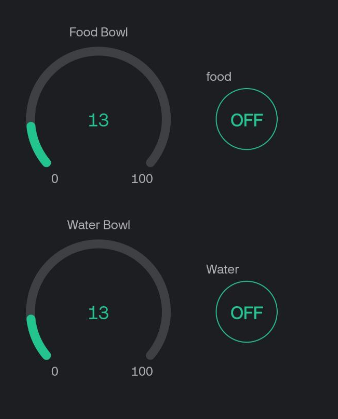
\includegraphics[width=80mm]{./Figuras/Desarrollo_Analisis/dash_vacios}
\caption{\textit{Dashboard} de Blynk con las tazas vacías.} 
\label{fig:analisis3}
\end{figure}

De este escenario A se puede analizar que se están imprimiendo lecturas de vacío esperadas. Esto indica que los sensores ultrasónicos están detectando adecuadamente cuando las tazas están vacías. El \textit{dashboard} muestra valores que concuerdan con lo que esta pasando en las tazas, por lo que la comunicación entre los sensores y el \textit{dashboard} funciona como se espera.

% CASO B llenando taza Agua X / Impresión en terminal X/ Foto del Dashboard X
\subsection{Caso B: Llenando taza Agua}
A continuación se analiza el escenario en el se acciona el botón de llenar taza de agua.

\begin{figure}[H]
\centering
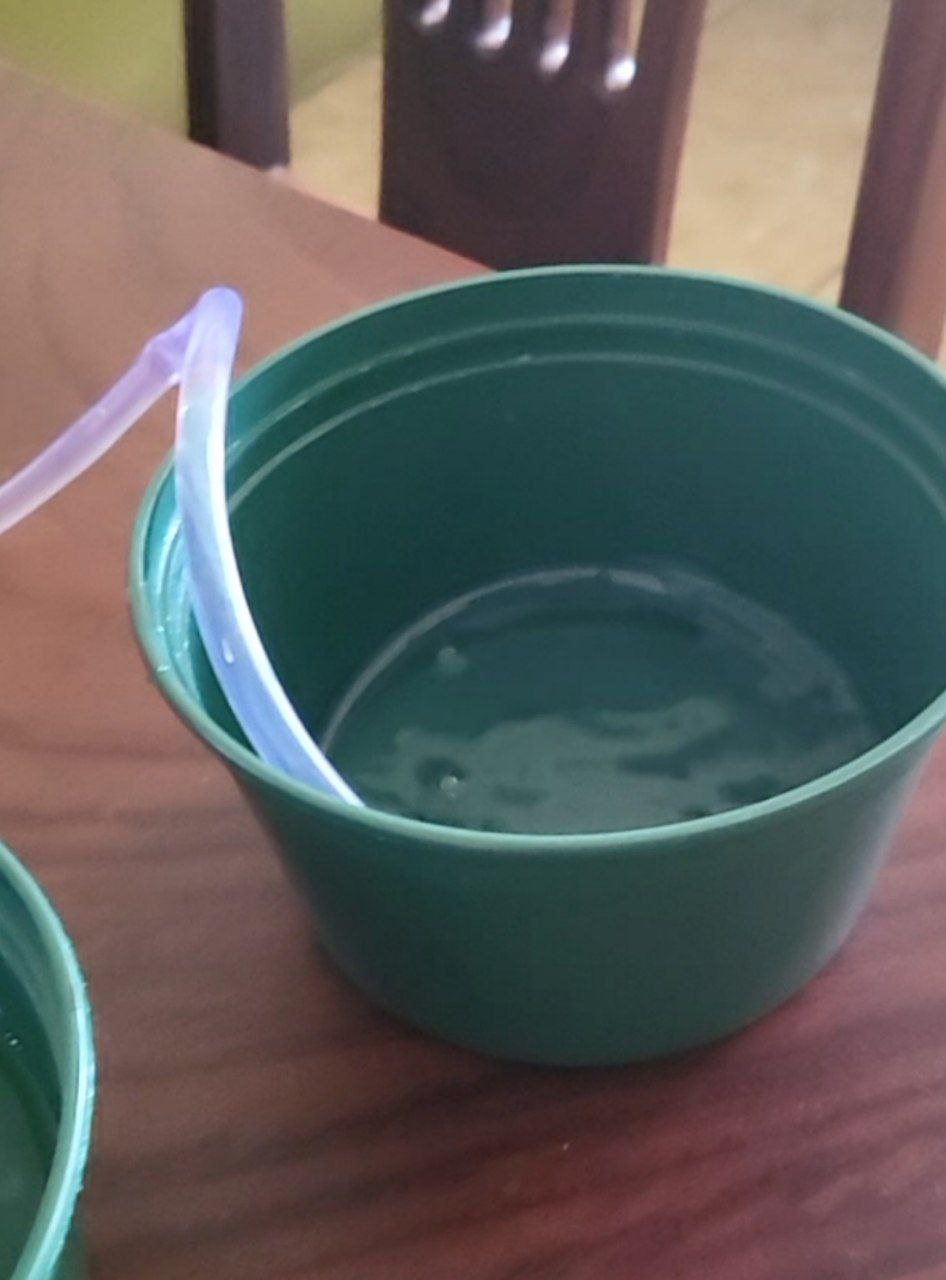
\includegraphics[width=80mm]{./Figuras/Desarrollo_Analisis/Llenado en progreso}
\caption{Imagen de taza de agua con el llenado en progreso.} 
\label{fig:analisis4}
\end{figure}
Mientras se esta realizando el llenado de la taza de agua, en terminal se obtiene la siguiente impresión:

\begin{figure}[H]
\centering
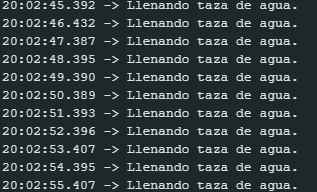
\includegraphics[width=80mm]{./Figuras/Desarrollo_Analisis/serial_llenando_agua}
\caption{Impresión con Serial monitor con llenado en progreso de taza de agua.} 
\label{fig:analisis5}
\end{figure}

A continuación una foto del \textit{dashboard} de Blynk con el llenado en progreso:

\begin{figure}[H]
\centering
\includegraphics[width=80mm]{./Figuras/Desarrollo_Analisis/Llenando agua}
\caption{\textit{Dashboard} con llenado en progreso de taza de agua.} 
\label{fig:analisis6}
\end{figure}

Al finalizar el llenado, se imprime lo siguiente en terminal:

\begin{figure}[H]
\centering
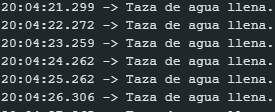
\includegraphics[width=80mm]{./Figuras/Desarrollo_Analisis/serial_agua_llena}
\caption{Impresión con Serial monitor con taza de agua llena.} 
\label{fig:analisis7}
\end{figure}
 
De este escenario, se observa un funcionamiento fluido y coherente entre los diferentes componentes del sistema. Al iniciar la acción desde Blynk, se verifica en el serial monitor que las impresiones de agua se realizan según lo esperado, confirmando que la bomba está operando correctamente. Además, en el \textit{dashboard} de Blynk se registra un progreso continuo y preciso en las mediciones de los niveles de agua, reflejando de manera efectiva el aumento en la cantidad de agua en la taza. Este escenario resalta la integración efectiva entre el control remoto mediante Blynk, la respuesta adecuada de los sensores y la visualización en tiempo real de los datos.

% CASO C llenando taza comida / Impresión en terminal X/ Foto del Dashboard X
\subsection{Caso C: Llenando taza de Comida}
A continuación se analiza el escenario en el se acciona el botón de llenar taza de comida

\begin{figure}[H]
\centering
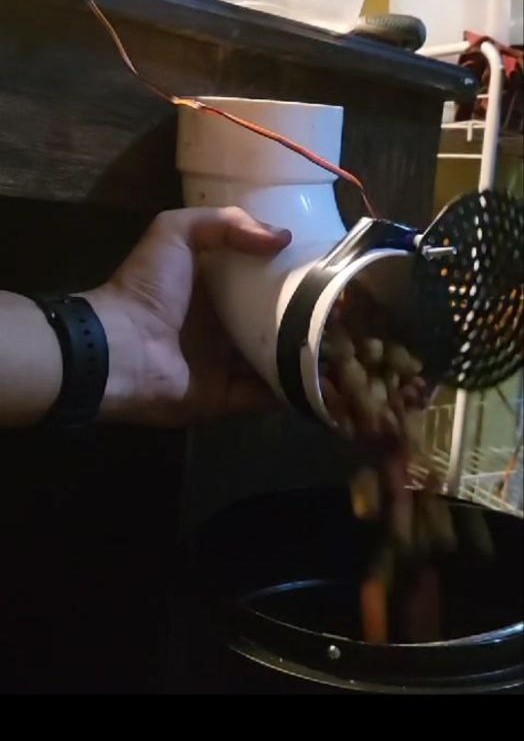
\includegraphics[width=80mm]{./Figuras/Desarrollo_Analisis/comida_progreso}
\caption{Imagen de Dispensador con llenado en progreso.} 
\label{fig:analisis8}
\end{figure}
Mientras se esta realizando el llenado de la taza de comida, en terminal se obtiene la siguiente impresión:

\begin{figure}[H]
\centering
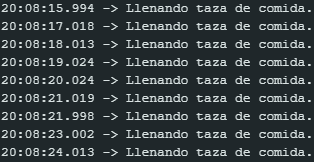
\includegraphics[width=80mm]{./Figuras/Desarrollo_Analisis/serial_llenando_comida}
\caption{Impresión con Serial monitor con llenado en progreso de taza de comida.} 
\label{fig:analisis9}
\end{figure}

A continuación una foto del \textit{dashboard} de Blynk con el llenado en progreso:

\begin{figure}[H]
\centering
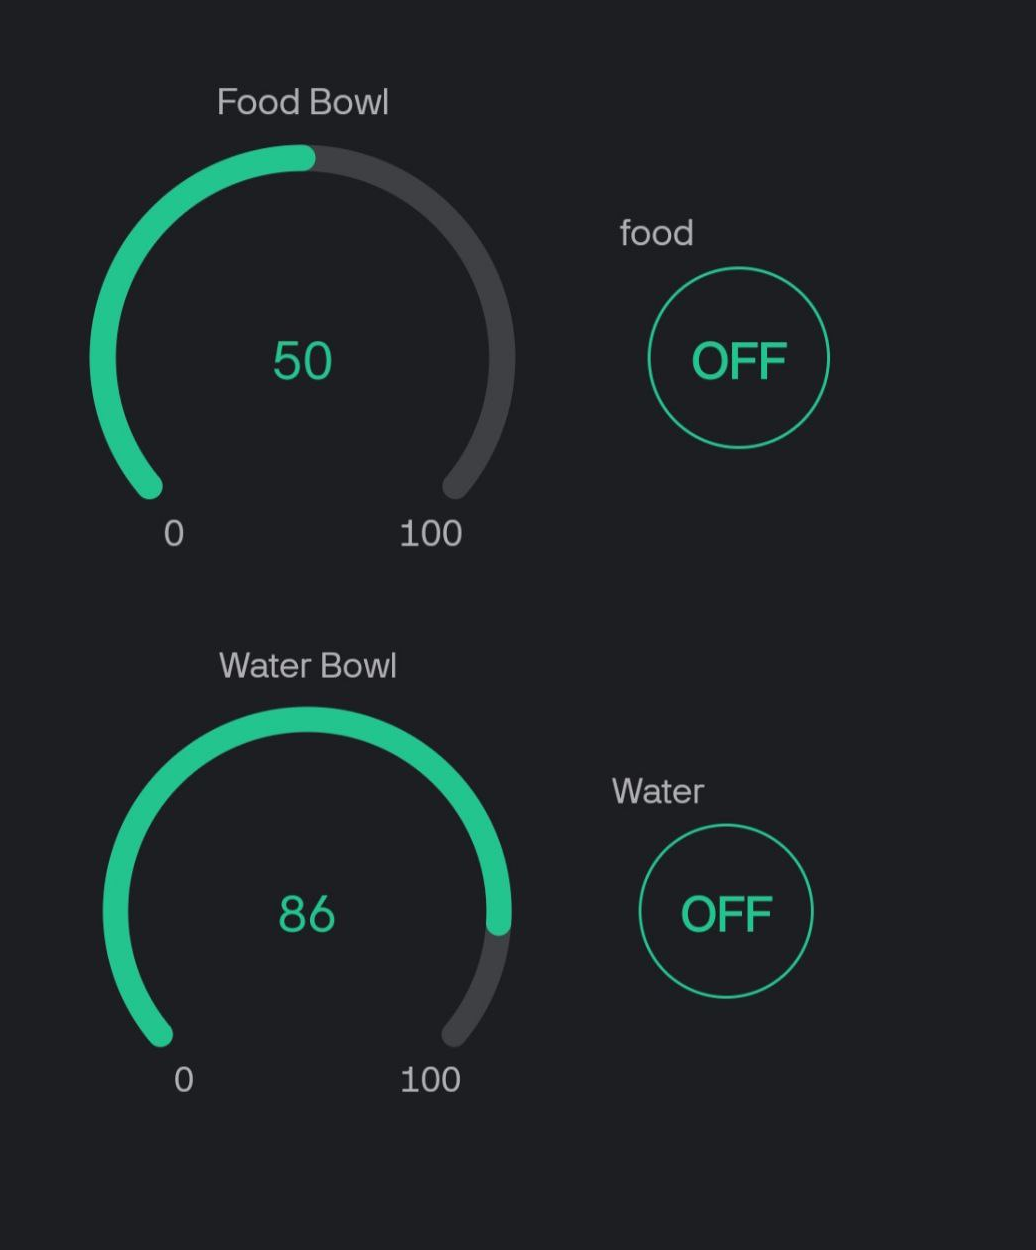
\includegraphics[width=80mm]{./Figuras/Desarrollo_Analisis/dash Llenando comida}
\caption{\textit{Dashboard} con llenado en progreso de taza de comida.} 
\label{fig:analisis10}
\end{figure}

Al finalizar el llenado, se imprime lo siguiente en terminal:

\begin{figure}[H]
\centering
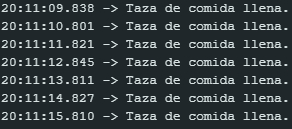
\includegraphics[width=80mm]{./Figuras/Desarrollo_Analisis/serial_comida_llena}
\caption{Impresión con Serial monitor con taza de comida llena.} 
\label{fig:analisis11}
\end{figure}
A continuación se muestra una imagen de ambas tazas llenas:

\begin{figure}[H]
\centering
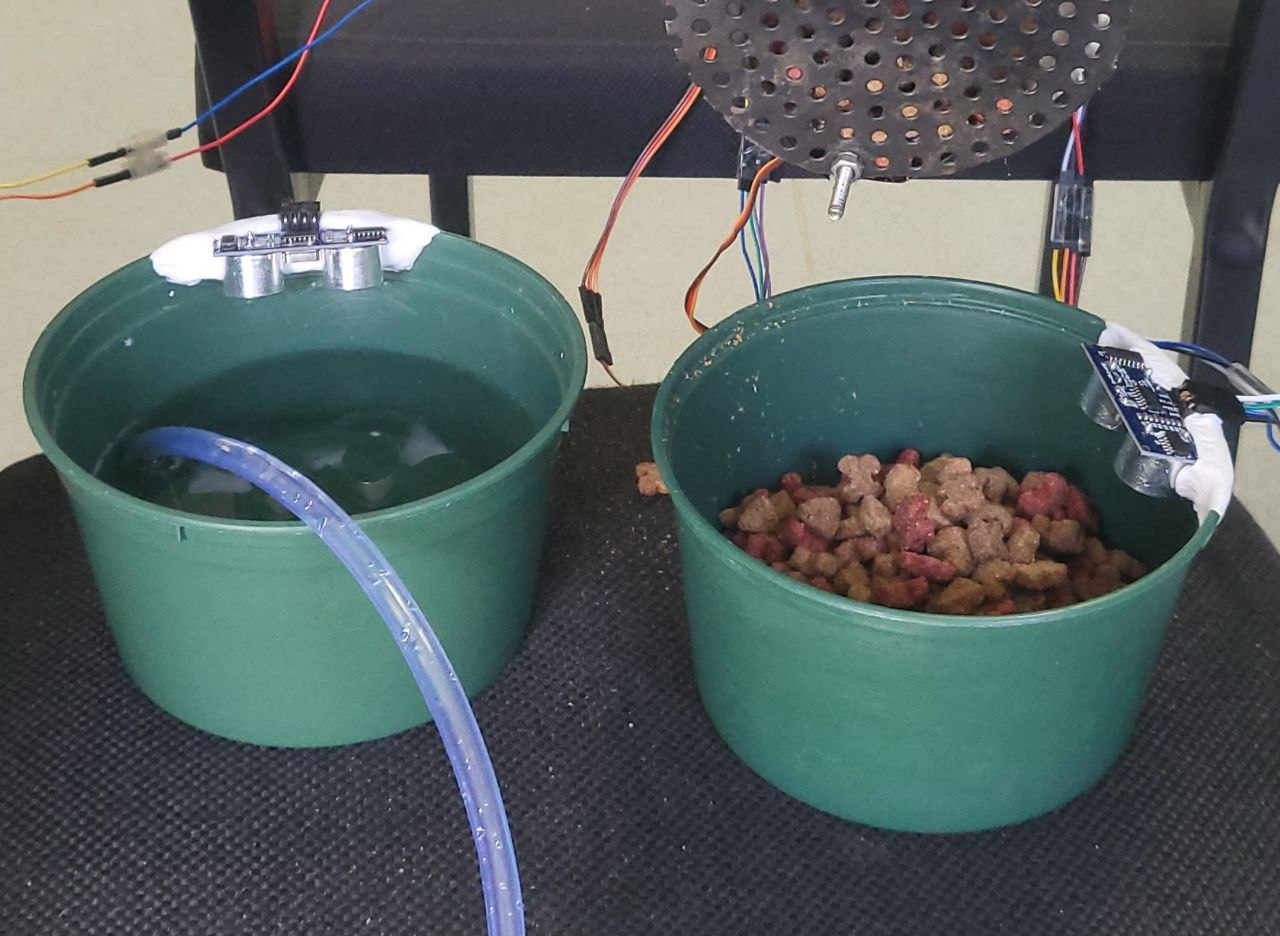
\includegraphics[width=80mm]{./Figuras/Desarrollo_Analisis/tazas_llenas}
\caption{Imagen del dispensador con tazas llenas.} 
\label{fig:analisis12}
\end{figure}

El \textit{dashboard} en este punto se muestra de la siguiente manera:

\begin{figure}[H]
\centering
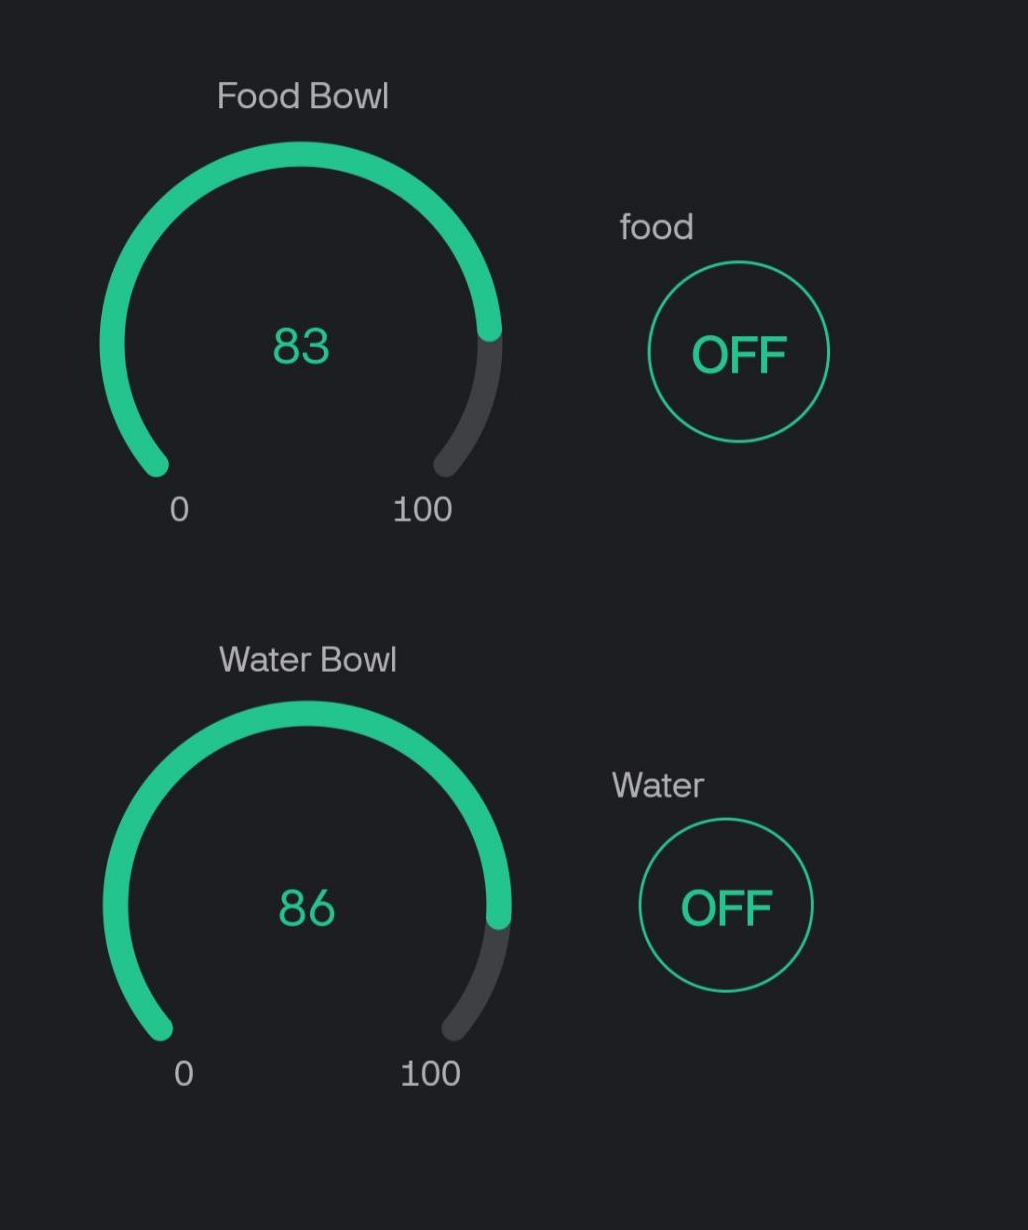
\includegraphics[width=80mm]{./Figuras/Desarrollo_Analisis/Ambos llenos}
\caption{\textit{Dashboard} con tazas llenas.} 
\label{fig:analisis13}
\end{figure}

De este ultimo escenario, se observa un desempeño robusto y coordinado del sistema. Al activar el servo motor a través de Blynk, el monitor serial proporciona retroalimentación en tiempo real con impresiones que indican el progreso del llenado, confirmando la operación adecuada del servo motor y la distribución de comida. El dashboard de Blynk refleja de manera precisa y progresiva el aumento en el nivel de comida en la taza, mostrando una sincronización efectiva entre la acción iniciada y la visualización de datos. 

\newpage
\section{CONCLUSIONES Y RECOMENDACIONES}
A lo largo del desarrollo del informe se pusieron a prueba una serie de conceptos y prácticas importantes para el manejo básico del ESP8266, para la construcción del sistemas de suministro de comida y agua para animales, utilizando IoT. A continuación algunas conclusiones y recomendaciones recolectadas a lo largo de trabajo realizado: 

\begin{itemize}
    \item A lo largo del proyecto, se realizaron ajustes importantes en el diseño y selección de componentes para cumplir con las prioridades definidas. La adaptación a las limitaciones técnicas, como el cambio de motores y la búsqueda de alternativas, permitió avanzar en el desarrollo del dispensador de comida y agua, logrando el objetivo principal del proyecto.

    \item El proyecto implicó enfrentar varios problemas técnicos, como la falta de potencia del ESP8266 y dificultades con Arduino Cloud. Se aplicaron estrategias efectivas, como la transición a Blynk, para superar estos obstáculos y garantizar el funcionamiento del sistema de dispensación de comida y agua, demostrando flexibilidad y capacidad de resolución.
    
    \item Se logró implementar funcionalidades básicas de IoT mediante la integración de Blynk, lo que permitió el monitoreo remoto del estado de los recipientes y el control del sistema desde un dispositivo móvil. Esta implementación cumplió parcialmente con el objetivo de automatización del suministro y facilitó el control a distancia del sistema.

    \item La construcción del hardware, que incluye el dispensador de comida, el sistema de bombas para agua y los sensores ultrasónicos, fue completada exitosamente. Este aspecto del proyecto proporcionó una base sólida para el funcionamiento básico del sistema, permitiendo que el dispensador cumpliera con sus funciones principales de manera efectiva.

    \item Para mejorar el rendimiento del servomotor y manejar mayores cargas, se recomienda replicar el circuito de relé. Este ajuste permitirá al servomotor operar con mayor potencia, lo cual es esencial para la dispensación efectiva de comida en el dispensador y para evitar problemas de desempeño.

    \item Se sugiere adaptar el diseño del dispensador en función del tipo de animal al que va dirigido. Ajustar el tamaño de los recipientes y el mecanismo de dispensación según las necesidades específicas del animal puede mejorar la eficacia del sistema y proporcionar una solución más adecuada para cada tipo de mascota.
\end{itemize} 

\input{05_Referencias}

\newpage
\section{Anexos}

\subsection{Hoja del fabricante del (...): información general} \label{an:01_GEN}
\vspace{\fill}
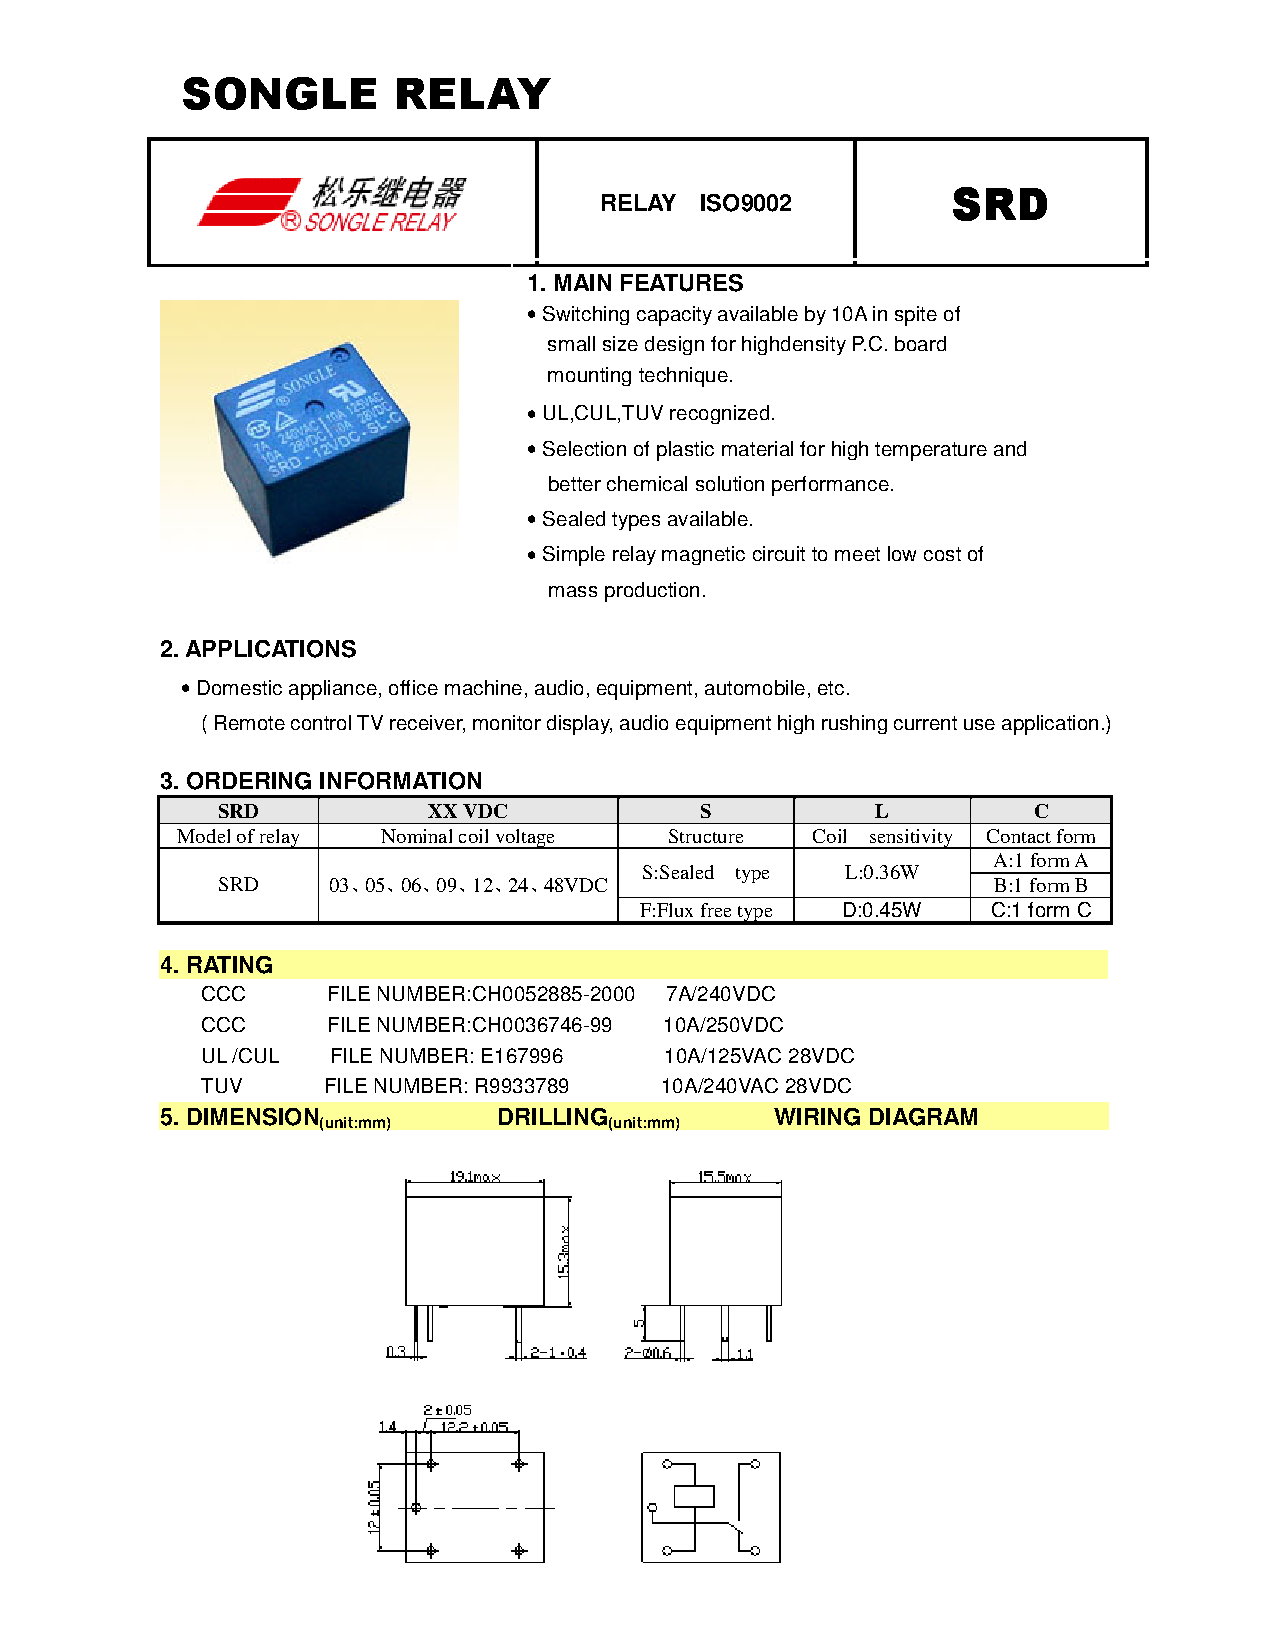
\includepdf[pages={1}]{./Documentos/Datasheet-RELE.pdf} 

\subsection{Hoja del fabricante del ESP8266: información general} \label{an:02_GEN}
\vspace{\fill}
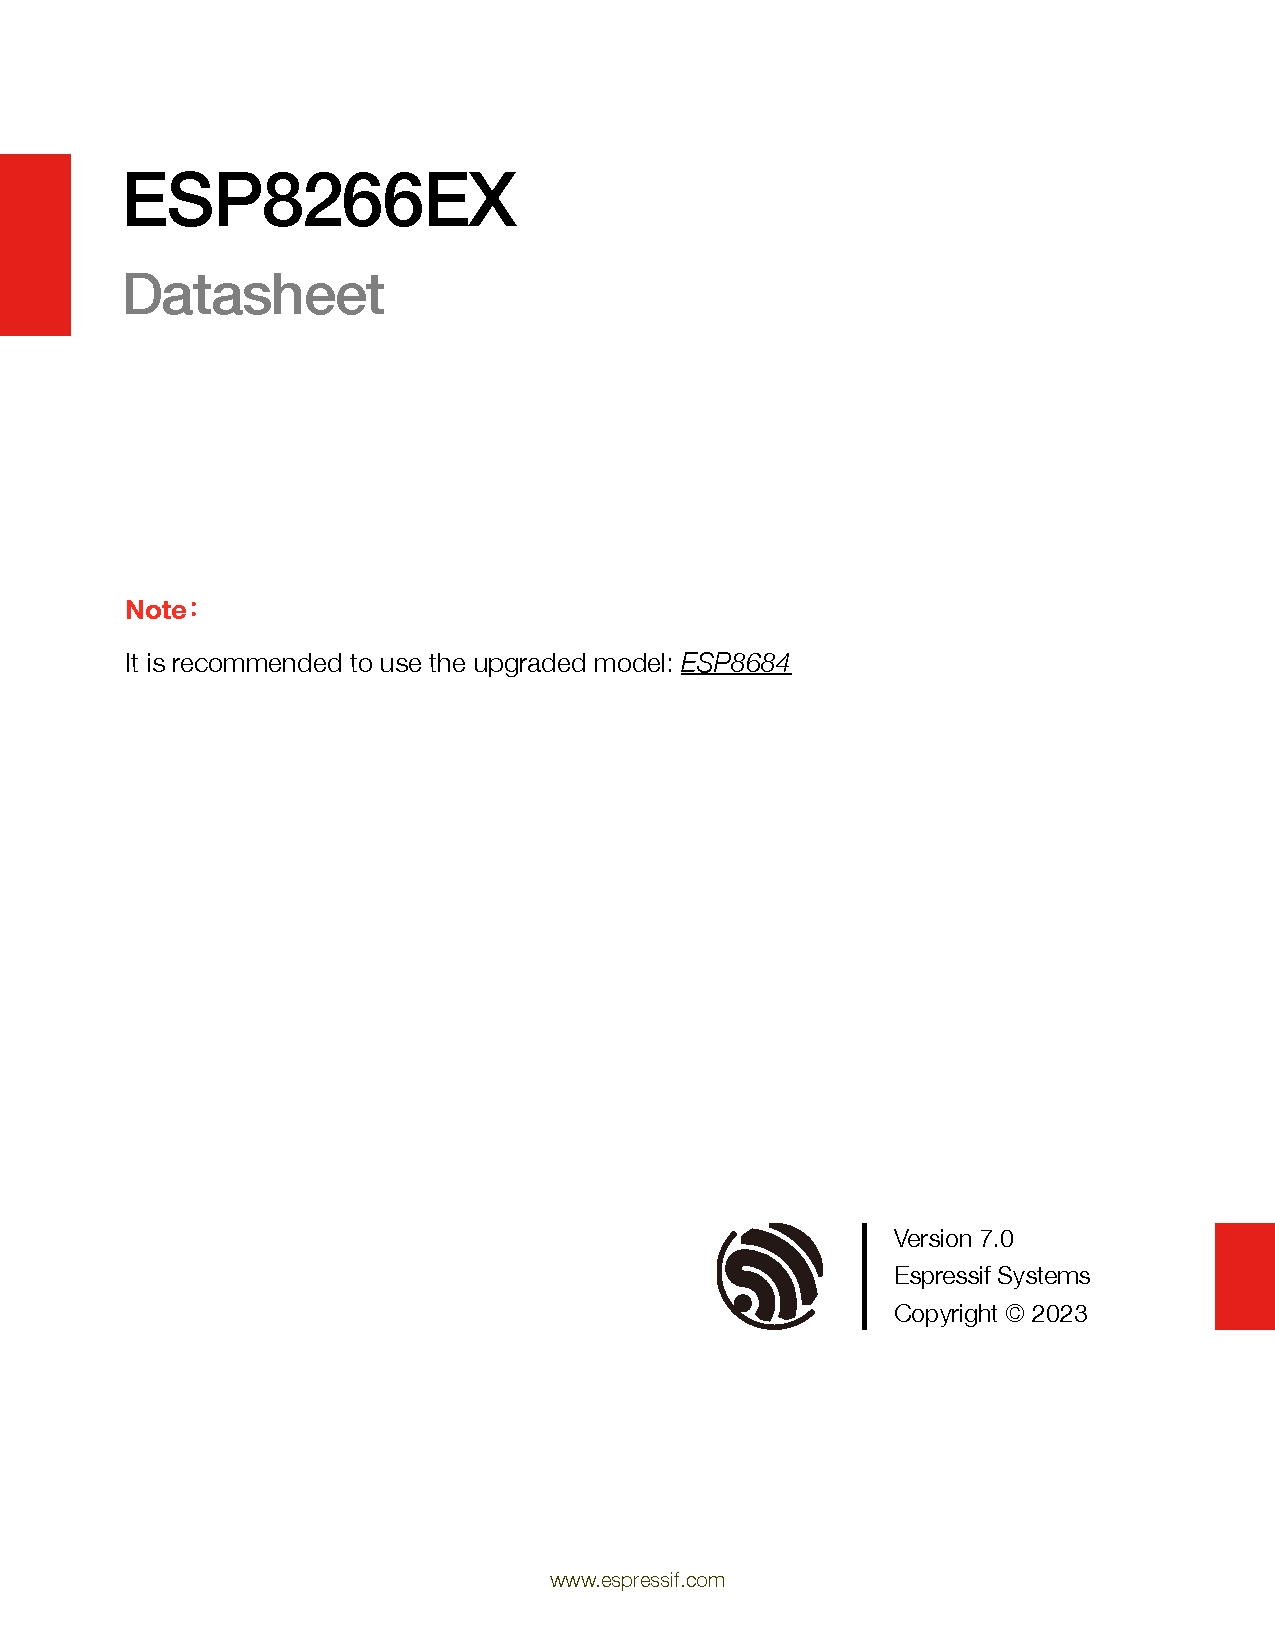
\includepdf[pages={1,7-24}]{./Documentos/ESP8266_DATASHEET.pdf} 


\end{document}

%Tareas pendientes en el informe

% ========== Introducción ========== %

% ========== Nota Teórica ========== % 

% ========== Desarrollo y Análisis de Resultados ========== % 

% ========== Conclusiones y recomendaciones ========== % 

% ========== Anexos ========== % 

# Tareas en Github 
% Crear la rama 
% Hacer un README básico 
% Subir el .ino
% Subir los archivos del informe y el PDF
